% World Wide Web journal (Springer, 11280) submission version.
% Uses the official sn-jnl.cls template downloaded from the journal's
% author kit (the template itself is bundled in the WW journal style).
% Single-blind review: author names go in \author (fill in before submitting).
\documentclass[pdflatex,sn-basic]{sn-jnl}

% Accept wider underfull tolerance to avoid noisy orphan/widow warnings on
% the WW journal template (which uses single-column A4 with generous margins).
\tolerance=10000
\emergencystretch=4em
\widowpenalty=10000
\clubpenalty=10000

\usepackage{graphicx}
\usepackage{booktabs}
\usepackage{amsmath}
\usepackage{amssymb}
\usepackage{amsthm}
\usepackage{algorithm}
\usepackage{algpseudocode}
\providecommand{\mathbbm}[1]{\mathbf{#1}}

% Theorem-class environments used in the method section.
% All numbered consecutively across the paper (per sn-jnl convention).
\newtheorem{hypothesis}{Hypothesis}
\newtheorem{theorem}{Theorem}
\newtheorem{lemma}{Lemma}
\newtheorem{corollary}{Corollary}
\newtheorem{definition}{Definition}
\newtheorem{remark}{Remark}

\graphicspath{{figures/}}
\begin{document}

\title[When Should Web-RAG Refresh?]{When Should Web-RAG Refresh? Adapting Refresh Policies Across Drift Regimes}

\author[1]{\fnm{Chaoyi} \sur{Guo}\textsuperscript{*}}\email{13293974463@163.com}
\author[1]{\fnm{Zhixing} \sur{Shi}\textsuperscript{*}}\email{zhixingshia@gmail.com}
\author[2]{\fnm{Jianyu} \sur{Zhou}\textsuperscript{*}}\email{2361010312@hhu.edu.cn}
\author[3]{\fnm{Zi'an} \sur{Wang}}\email{wangza2124@mails.jlu.edu.cn}
\author[4]{\fnm{Mingzhe} \sur{Liu}}\email{cnmingzheliu@outlook.com}
\author[1]{\fnm{Bohan} \sur{Zhang}}\email{qwertyu92024@163.com}
\author[1]{\fnm{Yu} \sur{Zhou}\textsuperscript{\dag}}\email{zhouyu@tyut.edu.cn}

\affil*[1]{\orgname{Taiyuan University of Technology}, \orgaddress{\city{Taiyuan}, \country{China}}}
\affil[2]{\orgname{Hohai University}, \orgaddress{\city{Nanjing}, \country{China}}}
\affil[3]{\orgname{Jilin University}, \orgaddress{\city{Changchun}, \country{China}}}
\affil[4]{\orgname{Shenzhen University}, \orgaddress{\city{Shenzhen}, \country{China}}}
\affil[ ]{\textsuperscript{*}These authors contributed equally to this work. \textsuperscript{\dag}Corresponding author: Yu Zhou (zhouyu@tyut.edu.cn).}

\maketitle

\section*{Abstract}
We study when a web-backed retrieval-augmented generation (RAG) system should refresh its cached evidence, and the answer depends on the corpus drift regime. Across two contrasting corpora, FreshQA (Wayback snapshots, low drift) and TimeVarying (our 60-query high-drift benchmark), separated by a large effect size in per-query content drift (Cohen's $d{=}1.94$, bootstrap 95\% CI $[1.18, 3.58]$), blind Always-Refresh inverts from the worst system on FreshQA (F1 $0.173$) to the best on TimeVarying (F1 $0.705$). No single fixed policy is right in both regimes, so we contribute two recipes. \textbf{AdaRefresh} is a DeBERTa-v3-small router proxy-trained on FreshQA freshness labels. It collapses zero-shot on the high-drift regime (F1 $0.422$) but $5$ mean-squared error (MSE) epochs on four labeled target queries recalibrate it to F1 $0.685$. The from-scratch control at the same budget plateaus at F1 $0.19$. \textbf{RegimeTest} averages a cheap drift predictor over ${\sim}20$ unlabeled queries and thresholds to pick the policy family, achieving complete separation of the two calibration corpora it was tuned on and reaching within $0.02$ of the fixed-policy best on either regime without any target labels; cross-corpus generalization of $\tau_{\text{regime}}$ is left to deployment-time calibration. A bounded channel decomposition and a direct FreshQA ablation attribute the low-drift cost of blind refresh to refreshed-evidence noise.

\begingroup
\flushleft
\textbf{Code:} \url{https://github.com/wu-mai/wise-rag-refresh}
\par
\endgroup

\begin{keywords}
Retrieval-augmented generation, Web information retrieval, Temporal query intent, Cache refresh, Domain adaptation, Cost-aware systems
\end{keywords}



\section{Introduction}
\label{sec:intro}

Web-RAG systems answer questions by retrieving web pages and conditioning a large language model (LLM) on the evidence. To keep latency and cost down, deployed systems cache retrieved pages; but the web is the system's source of truth and it does not sit still. Prices and leadership change, and every cached page ages against its live counterpart. The system therefore faces a per-query decision: answer from the cache, or pay for a live refresh of the evidence?

\begin{figure}[htbp]
\centering
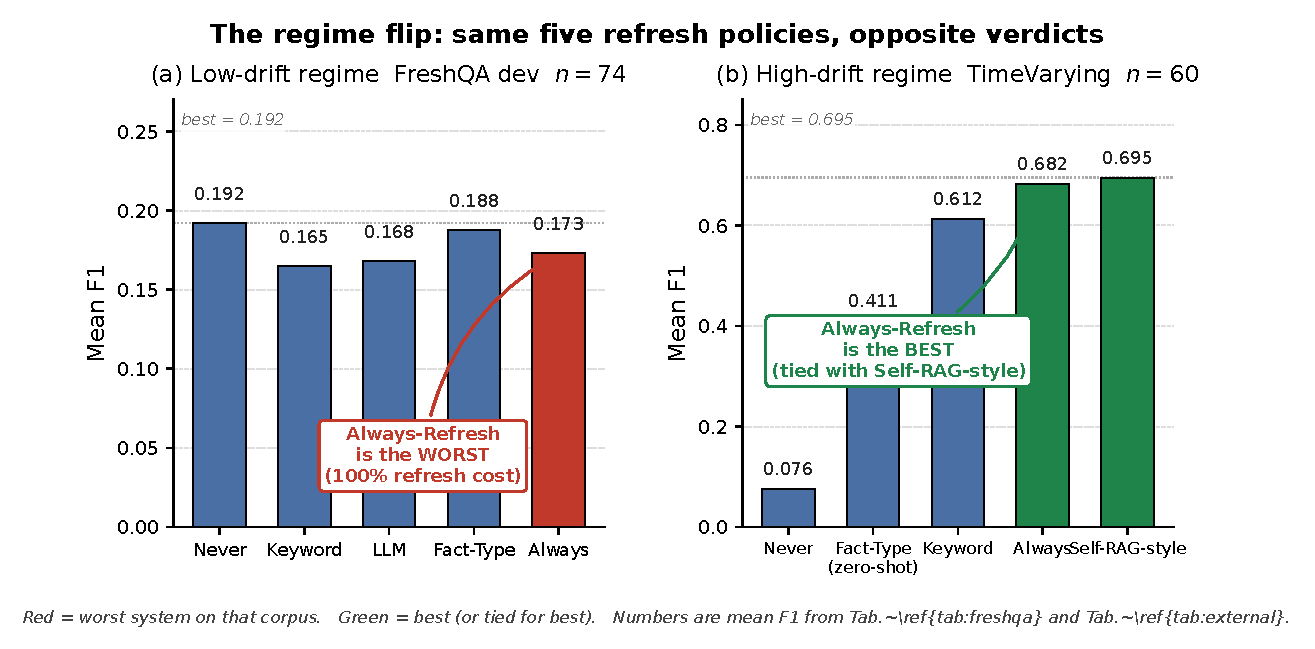
\includegraphics[width=\linewidth]{fig1_regime_flip.pdf}
\caption{The regime flip. The same five refresh policies (Never, Always, Keyword, LLM, Fact-Type Router) on two corpora: in the low-drift regime (left, FreshQA dev, $n{=}74$) blind Always-Refresh is the \emph{worst} system (F1 $0.173$ vs $0.192$ for Never) because refreshed evidence is a perturbation; in the high-drift regime (right, TimeVarying, $n{=}60$) it is the \emph{best} (F1 $0.705$ vs $0.191$) because stale evidence is simply wrong. Axes show mean token-level F1 against refresh rate. No fixed policy wins in both regimes, motivating a regime test (which family to ship) plus an adaptable router (the high-drift family's best member).}
\label{fig:frontier-intro}
\end{figure}

This decision has a price on both sides, and which side dominates is an empirical property of the corpus we call its \emph{drift regime} (Fig.~\ref{fig:frontier-intro}). When cached and current pages barely differ (low drift), refreshing buys nothing and can actively hurt: the fetched text perturbs the evidence the generator conditions on. When they differ substantively (high drift), skipping the refresh means answering from outdated evidence. A single fixed policy cannot be right in both regimes: as we show, blind Always-Refresh is the \emph{worst} system on a low-drift corpus (F1 $0.173$ vs $0.192$ for never refreshing) yet the \emph{best} on a high-drift one (F1 $0.705$ vs $0.191$).

Existing work stops short of this decision. Temporal-IR and freshness benchmarks~\cite{vu2023freshqa} measure \emph{how much} the web changes or \emph{when} stale context hurts, but do not learn a refresh policy; adaptive-retrieval methods~\cite{jiang2023flare,asai2023selfrag} decide whether to retrieve against a \emph{static} index and never condition on cache age; web-cache refresh heuristics optimize cache freshness and ignore downstream answer quality. Cost-aware refresh of RAG evidence, meaning the per-query decision of whether a live fetch is worth it and how that decision changes across drift regimes, remains unstudied at the system level.

We answer three questions on FreshQA (low drift, real Wayback snapshots~\cite{vu2023freshqa}) and a high-drift corpus we construct ($n{=}60$), separated by a large effect size in per-query content drift (Cohen's $d{=}1.94$, bootstrap 95\% CI $[1.18, 3.58]$): (RQ1) how much staleness hurts answer quality; (RQ2) does the best refresh policy depend on the drift regime; (RQ3) can a learned refresh router transfer across regimes and be repaired with few labels. Our method has three components, a \textbf{Freshness Router} that scores queries with a refresh probability, a \textbf{Refresh-aware Pipeline} that isolates evidence freshness from retrieval, and a \textbf{Few-shot Adaptation} step. Two recipes emerge from this stack:
\begin{itemize}
  \item \textbf{AdaRefresh} (transfer-and-adapt): a proxy-trained router collapses zero-shot across regimes (F1 $0.422$); $5$ epochs of adaptation on $k{\ge}4$ target queries recovers it to $0.685$, above every rule-based policy. The from-scratch control at the same budget plateaus at $0.19$: the gain comes from the proxy prior.
  \item \textbf{RegimeTest} (regime classification): averaging a cheap drift predictor over ${\sim}20$ held-out queries separates the two regimes with no overlap and selects the policy family within $0.02$ of the fixed-policy best. It answers \emph{which} policy to ship.
\end{itemize}

Our contributions:
\paragraph*{Contributions}
\textbf{AdaRefresh} is a transfer-and-adaptation method for refresh routing: a proxy-trained DeBERTa router that collapses zero-shot across drift regimes is recalibrated with $5$ epochs of MSE adaptation saturating at $k{=}4$; the from-scratch control at the same budget isolates the proxy prior as the source of the gain, and leave-one-category-out (LOCO) cross-validation rules out memorization.
\medskip
\textbf{RegimeTest} is a corpus-level regime classifier: averaging a sub-$100$-parameter drift predictor over ${\sim}20$ unlabeled deployment queries separates low- and high-drift regimes with no classification error across five seeds and the two calibration corpora; the threshold $\tau_{\text{regime}}$ is calibrated on the target corpus, so cross-corpus generalization is an open question we leave to deployment-time tuning.
\medskip
\textbf{A controlled decomposition} of the regime flip: a bounded cross-table argument corroborated by a direct FreshQA ablation attributes the low-drift cost of blind refresh to refreshed-evidence noise.
\medskip
\textbf{Resources}: the TimeVarying benchmark (60 queries, 5 categories, stale/fresh evidence pairs) and the full pipeline code, released for reproducibility.
\section{Related Work}
\label{sec:related}

\subsubsection*{Temporal retrieval and web freshness.}~Time-aware ranking and recency-sensitive retrieval model \emph{when} documents are relevant. FreshQA~\cite{vu2023freshqa} supplies time-sensitive QA data and labels (e.g., \texttt{never}-, \texttt{slow}-, \texttt{fast-changing}) but does not study refresh \emph{policies}. Recent work estimates how recent evidence must be, diagnoses when stale context hurts generation, and benchmarks agents on evolving knowledge. None of these works study cost-aware refresh or how refresh policies transfer across drift regimes, which is the gap our work targets.

\subsubsection*{Adaptive retrieval and cross-corpus transfer.}~Self-RAG~\cite{asai2023selfrag}, CRAG~\cite{crag2024}, RAPTOR~\cite{raptor2024}, FLARE~\cite{jiang2023flare}, and SeaKR~\cite{seakr2025} decide \emph{whether or when} to retrieve from a static index; they treat the corpus as static and do not condition on corpus \emph{age}. BEIR~\cite{thakur2021beir} showed that dense retrievers transfer unevenly across corpora, and we apply the same observation to the refresh-policy setting. Calibrated retrieval-budget allocation is adjacent but does not address live-refresh cost. Our work isolates when selective live-refresh against a stale cache helps, and when proxy-trained routers fail to transfer across drift regimes.

\subsubsection*{Cache refresh and our position relative to it.}~Classical web-cache refresh~\cite{bingyuan2017cache} and time-to-live (TTL) heuristics optimize \emph{freshness of the cache} as the objective, with staleness versus refresh frequency as the trade-off. RAG refresh is a different problem: the unit of work is the \emph{answer quality of a downstream LLM}, and the trade-off is between that quality and refresh cost (latency, dollars). The cache-refresh literature has no notion of an LLM-conditioned reader, and an LLM-conditioned reader is sensitive to \emph{which} document changes, not just \emph{whether} something has changed: a refreshed Wikipedia paragraph can introduce a stylistic or topical shift that hurts answer quality even when the gold answer is unchanged. Our regime-dependent result is therefore not derivable from TTL heuristics: in the low-drift setting, blind refresh \emph{worsens} answer quality even though it strictly improves freshness, the opposite of what a TTL policy would predict.

\subsubsection*{Transfer learning and low-shot adaptation.}~Transfer-and-adapt recipes are well-studied in NLP~\cite{howard2018ulmfit,devlin2019bert} and have been used to recalibrate ranking models across corpora~\cite{thakur2021beir}. Our adaptation step is in this lineage but specialized in two ways. The target supervision is not a label but a scalar \emph{refresh utility}, and the model is a small regression head on top of a frozen-source representation. The sample-flat saturation we observe ($k{=}4$ already covers most of the gain) is consistent with the low-dimensional calibration view we develop in §\ref{sec:interpretive}.

\subsubsection*{Positioning relative to existing systems.}~The closest published systems are Self-RAG~\cite{asai2023selfrag}, FLARE~\cite{jiang2023flare}, SelfAsk~\cite{press2022measuring}, IRCoT~\cite{trivedi2023interleaving}, the FreshLLMs/FreshQA study~\cite{vu2023freshllms}, and CRAG~\cite{crag2024}. All six decide when to retrieve, or how to condition answer generation, against an open or live search corpus. Our setup differs in three ways. (i) The decision object: they route retrieval against a live index, we decide whether to refresh a stale cache. (ii) The supervision budget: their routers train on hundreds to thousands of labeled examples; ours adapts with $4{-}60$ labeled queries. (iii) The evaluation regime: they report search-augmented QA accuracy with GPT-4 or LLaMA backbones; we report conditional F1 on stale-vs-fresh evidence pairs with GPT-5.4, so direct F1 comparison is not meaningful. As an internal anchor, we reproduced a Self-RAG-style prompt router inside our pipeline with one LLM call per query; it reaches F1 $0.695$ on TimeVarying, within seed variance ($\sigma \approx 0.06$ across our 3-seed label-efficiency runs) of our adapted AdaRefresh router at $0.685$ (§\ref{sec:rq2}, Table~\ref{tab:external}). A shared refreshed-evidence benchmark would enable a direct head-to-head comparison; building one is left to future work.

\section{Method}
\label{sec:method}

\begin{figure}[!t]
\centering
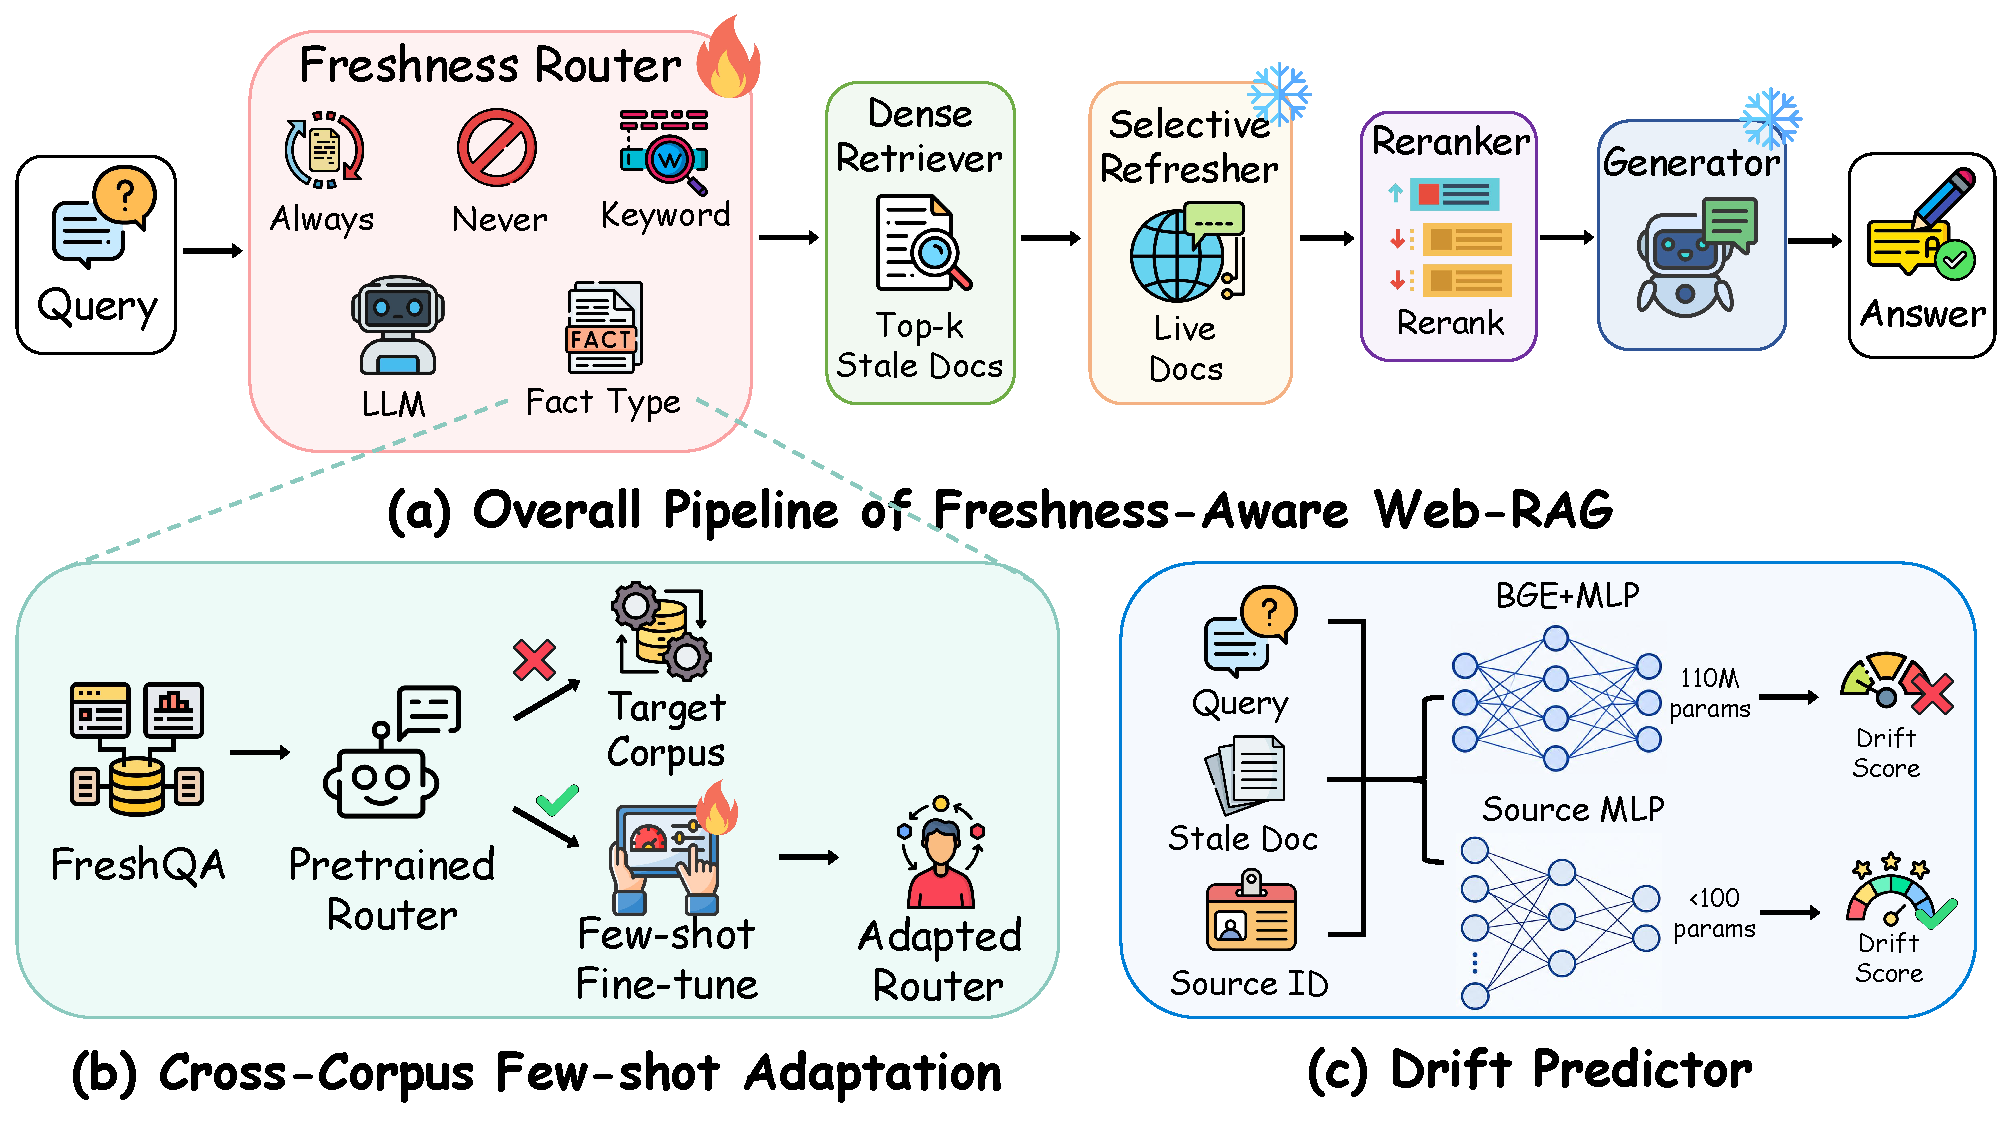
\includegraphics[width=0.82\linewidth]{framework_webrag.pdf}
\caption{Overall framework of the freshness-aware Web-RAG pipeline: the \emph{Freshness Router} (§\ref{sec:drift-aware}) scores each query, the \emph{Refresh-aware Pipeline} (§\ref{sec:method-pipeline}) selectively refreshes and reranks, and the \emph{Few-shot Adaptation} step (§\ref{sec:adapt-objective}) recalibrates the router to a new corpus with a handful of labels.}
\label{fig:method-framework}
\end{figure}

\subsection{Problem Formulation and Method Overview}
\label{sec:method-overview}

A Web-RAG system answers queries against a cached web corpus. Cached pages age while the web moves, so before answering a query $q_t$ the system chooses an action $a_t \in \{\texttt{Reuse}, \texttt{Refresh}\}$: refresh fetches the current version of the candidate documents (a real cost, paid in latency and fetch traffic), reuse answers from the cache. The system's goal is to maximize answer quality (token-level F1) at a bounded refresh rate. Formally, a policy $\pi$ chooses $a_t$ from pre-answer features $x_t$ and we evaluate the pair $\big(\text{mean } F_1,\ \mathrm{RR}(\pi)\big)$ where $\mathrm{RR}(\pi)=\frac{1}{T}\sum_t \mathbb{E}_{a_t\sim\pi}[a_t]$ is the average refresh rate; a scalar trade-off $F_1 - \lambda\,\mathrm{RR}$ with weight $\lambda$ recovers the standard quality--cost objective.

\paragraph*{Notation.}~All symbols used throughout the paper are fixed in Table~\ref{tab:notation}; every downstream equation is written using only these names.
\begin{table}[htbp]
\centering
\small
\caption{Notation used throughout the paper. Subscript $t$ indexes the query stream; subscript $i$ indexes the $k$-shot target set; superscripts $\mathrm{s}$/$\mathrm{f}$ mark stale and fresh variants.}
\label{tab:notation}
\centering
\renewcommand{\arraystretch}{1.05}
\begin{tabular}{llp{9.4cm}}
\toprule
Symbol & Type & Meaning \\
\midrule
$q$ & query & a user query, drawn from the corpus query distribution $P_{\mathcal{C}}$ \\
$e^{\mathrm{s}}_i,\, e^{\mathrm{f}}_i$ & evidence & stale and fresh evidence documents for query $q_i$ \\
$\mathcal{C}$ & corpus & the cached web corpus (a multiset of stale documents) \\
$\delta_i \in [0,1]$ & drift & per-query drift $\delta_i := 1 - \mathrm{Jaccard}(e^{\mathrm{s}}_i, e^{\mathrm{f}}_i)$ \\
$\bar\delta,\, \sigma_\delta$ & drift & corpus-mean drift and its empirical std \\
$x_t \in \mathbb{R}^{6}$ & feature & six stale-side features of query $q_t$ (Table~\ref{tab:features}) \\
$\Phi(q, e^{\mathrm{s}})$ & map & feature extractor producing $x$ (Eq.~\ref{eq:feature-map}) \\
$f_\theta : \mathbb{R}^{6} \to \mathbb{R}$ & map & drift predictor with parameters $\theta$ \\
$\hat\delta_t \triangleq f_\theta(x_t)$ & score & predicted per-query drift \\
$p_{\mathrm{fresh}}(x_t) \in [0,1]$ & score & refresh probability (Eq.~\ref{eq:pfresh}) \\
$a_t \in \{0,1\}$ & action & refresh decision ($1$ = refresh, $0$ = reuse) \\
$\pi : \mathcal{X} \to \{0,1\}$ & policy & refresh policy; $\pi(x) = \mathbb{1}\{p_{\mathrm{fresh}}(x) > \tau\}$ (Eq.~\ref{eq:router}) \\
$\tau,\, \tau^\star_\lambda$ & scalar & decision threshold; $\tau^\star_\lambda$ maximizes $F_1 - \lambda\cdot\mathrm{RR}$ on validation \\
$\boldsymbol\beta = (\beta_1, \beta_2)$ & weights & reranker freshness-bonus weights (Eq.~\ref{eq:rerank}); distinct from $\lambda$ \\
$\lambda \ge 0$ & scalar & refresh-cost weight in the scalarized objective \\
$\mathrm{RR}(\pi)$ & metric & refresh rate $\mathrm{RR}(\pi) := T^{-1} \sum_{t} \pi(x_t)$ \\
$F_1(q; \pi)$ & metric & token-level F1 of the generator given policy $\pi$ \\
$u_t(a) := F_1(q_t; a) - \lambda \cdot a$ & utility & per-query utility (Eq.~\ref{eq:utility}) \\
$\pi^\star$ & policy & Bayes-optimal refresh policy (Eq.~\ref{eq:bayes-policy}) \\
$R(\pi)$ & metric & expected regret of $\pi$ against $\pi^\star$ (Eq.~\ref{eq:regret}) \\
$\tilde y_i \in \{0,1\}$ & label & target supervision ($1$ = freshness-sensitive) \\
$\mathcal{D}^{\mathrm{tar}}_k = \{(x_i, \tilde y_i)\}_{i=1}^{k}$ & set & $k$-shot target adaptation set \\
$\theta_{\mathrm{src}},\, \theta_{\mathrm{adapt}}$ & params & source-trained and adapted router parameters \\
$L$ & constant & Lipschitz constant of $F_1(\cdot)$ with respect to $\delta$ \\
$r$ & integer & intrinsic dimension of the corpus-shift subspace (Hypothesis~\ref{hyp:lowdim}) \\
$\hat c \in \{0,1\}$ & label & corpus-level regime classification ($0$ = low-drift, $1$ = high-drift) \\
$\overline{\hat\delta} := \frac{1}{B}\sum_{i=1}^{B} \hat\delta_i$ & score & batch-mean predicted drift over $B$ unlabeled queries \\
$\tau_{\mathrm{regime}}$ & scalar & regime-classifier threshold; midpoint of training-fold corpus means \\
\bottomrule
\end{tabular}
\end{table}

\paragraph*{Objective and Bayes-optimal policy.}~With the notation above, the scalarized objective is
\begin{equation}
\label{eq:tradeoff}
\max_{\pi}\,\mathbb{E}_{q \sim P_{\mathcal{C}}}\big[\, F_1(q;\,\pi) \;-\; \lambda\cdot\mathrm{RR}(\pi)\,\big],
\end{equation}
and the per-query utility of taking action $a \in \{0,1\}$ is
\begin{equation}
\label{eq:utility}
u_t(a) \;:=\; F_1(q_t;\,a) \;-\; \lambda\cdot a.
\end{equation}
The Bayes-optimal refresh rule compares the expected utility of refreshing against that of reusing the cache:
\begin{equation}
\label{eq:bayes-policy}
\pi^\star(q) \;:=\; \mathbb{1}\!\left\{\,\mathbb{E}\!\left[\,F_1(q;\,a{=}1,\,e^{\mathrm{f}}) - F_1(q;\,a{=}0,\,e^{\mathrm{s}})\,\right] \;\ge\; \lambda\,\right\}.
\end{equation}
\noindent Eq.~\ref{eq:bayes-policy} is unobservable in practice (it requires knowing the gold answer), so the rest of the paper designs observable proxies $\hat\pi$ that approximate $\pi^\star$ at low label cost.

Our method consists of three named components (Fig.~\ref{fig:method-framework}):
\begin{itemize}
  \item \textbf{Freshness Router} (§\ref{sec:drift-aware}): a DeBERTa regressor that scores each query with a refresh probability $p_{\mathrm{fresh}} \in [0,1]$ from six stale-side features, thresholded into a refresh decision;
  \item \textbf{Refresh-aware Pipeline} (§\ref{sec:method-pipeline}): same-URL selective refresh + freshness-bonus reranking + a fixed generator, so that all F1 differences are attributable to refresh decisions;
  \item \textbf{Few-shot Adaptation} (§\ref{sec:adapt-objective}): a $5$-epoch MSE recalibration of the router on as few as $k{=}4$ target-corpus queries.
\end{itemize}
Beyond the algorithm, two lightweight \emph{interpretive models}, a low-dimensional-calibration hypothesis and a regret bound, explain \emph{why} the adaptation works (§\ref{sec:interpretive}); they are not pipeline components.

\subsection{Freshness Router}
\label{sec:drift-aware}

The router scores each query with a refresh probability from six stale-side scalar features $x_t \in \mathbb{R}^{6}$ (Table~\ref{tab:features}). All six are computable \emph{before} answering, from the query text and the cached evidence alone:

\begin{table}[htbp]
\caption{The six stale-side features of the Freshness Router. All are computed from the query and the \emph{cached} evidence; none requires a live fetch.}
\label{tab:features}
\centering
\small
\begin{tabular}{llp{7.2cm}}
\toprule
\# & Feature & Rationale \\
\midrule
1 & query length & long queries tend to specify more context, less open-ended facts \\
2 & $\log(1{+}$query length$)$ & compresses the length distribution's heavy tail \\
3 & evidence length & long cached pages are more likely to contain the answer already \\
4 & $\log(1{+}$evidence length$)$ & same compression for the evidence side \\
5 & query--evidence overlap & Jaccard overlap of content words; high overlap means the cache likely answers the query as-is \\
6 & temporal novelty & indicator for cues such as \emph{current}, \emph{latest}, \emph{today}, explicit years; the single most predictive feature \\
\bottomrule
\end{tabular}
\end{table}

A drift predictor $f_\theta$ maps the features to a scalar drift score $\hat\delta_t$, and a calibration head turns it into the refresh probability:
\begin{equation}
\label{eq:feature-map}
x \;:=\; \Phi(q,\,e^{\mathrm{s}}) \;\in\; \mathbb{R}^{6},
\end{equation}
\begin{equation}
\label{eq:drift-score}
\hat\delta_t \;:=\; f_\theta(x_t) \;=\; w_d^{\top} x_t + b_d \qquad \text{(Source MLP instantiation)},
\end{equation}
\begin{equation}
\label{eq:pfresh}
p_{\mathrm{fresh}}(x_t) \;=\; \sigma\!\big(w^\top x_t + u\, f_\theta(x_t) + b\big),
\end{equation}
where $\sigma$ is the sigmoid. The drift score has two instantiations (Fig.~\ref{fig:method-framework}c): a \emph{Source MLP} (multi-layer perceptron) with under $100$ parameters over the six features, cheap and transparent, which survives in the deployment pipeline as the engine of the corpus-level regime classifier (§\ref{sec:rq2-regime}); and a \emph{BGE+MLP} variant (${\sim}110$M parameters) over dense embeddings, which is more expressive but sample-hungry and underperforms at our label budgets (§\ref{sec:rq3}), so we evaluate it only as an ablation. The main learned instantiation replaces the hand-crafted head with a DeBERTa-v3-small~\cite{deberta2021} regressor that consumes the raw query and outputs $p_{\mathrm{fresh}}(q)$ directly. It is proxy-trained on FreshQA's \texttt{fact\_type} metadata: each training query carries a freshness label mapped to a regression target (\texttt{never-changing} $\to 0.0$, \texttt{slow-changing} $\to 0.5$, \texttt{fast-changing} $\to 1.0$), and the model is optimized with the MSE objective of Eq.~\eqref{eq:mse-loss} for $6$ epochs of AdamW (lr $2{\times}10^{-5}$, batch $16$, max length $64$). At inference the router is a single local forward pass per query, orders of magnitude cheaper than a per-query LLM call. The decision is the thresholded score
\begin{equation}
\label{eq:router}
a_t \;=\; \mathbbm{1}\{p_{\mathrm{fresh}}(x_t) > \tau\},
\end{equation}
with $\tau$ selected on validation data to maximize $F_1 - \lambda\cdot\mathrm{RR}$, following the standard selective-prediction pattern~\cite{geifman2017selective} with refresh as the ``abstain'' action.

\subsubsection*{Why six scalar features.}~Refresh routing is a \emph{calibration} problem over a few operational statistics, not a semantic matching problem: we hypothesize the refresh gain depends on a low-dimensional state $\Delta_t \approx h(Px_t)$, and estimation error in the full embedding space scales as $\mathcal{O}(\sqrt{d_{\mathrm{eff}}/n})$ in effective dimension $d_{\mathrm{eff}}$ and label count $n$; at our $n$, compact features beat expressive ones (§\ref{sec:rq3}; the BGE+MLP variant underperforms).

\subsection{Refresh-aware Pipeline}
\label{sec:method-pipeline}

The pipeline is deliberately fixed so that differences across refresh policies are attributable to refresh decisions alone (Fig.~\ref{fig:method-framework}). A query flows through four stages. \emph{(i) Routing}: the policy of Eq.~\eqref{eq:router} scores the query. \emph{(ii) Stale retrieval}: BGE-base~\cite{bge2023} retrieves the top-$m$ candidates from the cached index,
\begin{equation}
\label{eq:retrieval}
\mathcal{R}(q) \;:=\; \mathrm{top}\text{-}m\;\mathrm{BGE}(q,\,\mathcal{C}), \qquad m = 3.
\end{equation}
\emph{(iii) Selective refresh}: for triggered queries, refresh performs \emph{same-URL replacement}: the current version of a cached document replaces it in the same slot, so the candidate set and retrieval scores are unchanged and only the evidence text can differ; this isolates evidence freshness from retrieval coverage. \emph{(iv) Rerank and generate}: the reranker combines retrieval scores with freshness indicators,
\begin{equation}
\label{eq:rerank}
s_{\mathrm{final}}(d) \;=\; s_{\mathrm{retrieval}}(d) \;+\; \beta_1\,\mathbbm{1}_{\mathrm{live}}(d) \;+\; \beta_2\,\mathbbm{1}_{\mathrm{changed}}(d),
\end{equation}
with freshness-bonus weights $\boldsymbol\beta = (\beta_1, \beta_2)$, distinct from the trade-off weight $\lambda$; and the generator (fixed across all systems) answers from the top-3,
\begin{equation}
\label{eq:generate}
\hat y \;\sim\; \mathcal{G}\!\left(\,\mathrm{rerank}_{\boldsymbol\beta}\!\big(\mathcal{R}(q)\big)\,\right).
\end{equation}
The five refresh policies studied in this paper differ only in the router of Eq.~\eqref{eq:router}: (i)~\emph{Never Refresh} outputs $0$; (ii)~\emph{Always Refresh} outputs $1$; (iii)~\emph{Keyword Router} fires on temporal cues; (iv)~\emph{LLM Router} asks a zero-shot LLM; (v)~\emph{Fact-Type Router} is the learned router of §\ref{sec:drift-aware}.

\subsection{Few-shot Adaptation}
\label{sec:adapt-objective}

A proxy-trained router (e.g., on FreshQA's \texttt{fact\_type} labels) collapses zero-shot on a new corpus because its output scale matches the source drift distribution rather than the target one. Adaptation repairs this with a handful of target labels $\mathcal{D}^{\mathrm{tar}}_k = \{(x_i, \tilde y_i)\}_{i=1}^{k}$. The two-phase procedure is given in Algorithm~\ref{alg:adarefresh}.

\begin{algorithm}[htbp]
\caption{AdaRefresh: proxy-train on source, adapt on $k$ target labels.}
\label{alg:adarefresh}
\begin{algorithmic}[1]
\State \textbf{Input:} source set $\mathcal{D}_{\mathrm{src}}$ (FreshQA \texttt{fact\_type} labels), target set $\mathcal{D}^{\mathrm{tar}}_k = \{(x_i, \tilde y_i)\}_{i=1}^{k}$, learning rates $\eta_{\mathrm{src}}, \eta_{\mathrm{adapt}}$, epochs $E_{\mathrm{src}}, E_{\mathrm{adapt}}$.
\State \textbf{Phase 1 (proxy pre-training):} $\theta_{\mathrm{src}} \gets \arg\min_\theta \sum_{i \in \mathcal{D}_{\mathrm{src}}} \big(p_\theta(x_i) - y_i^{\mathrm{FreshQA}}\big)^2$ over $E_{\mathrm{src}}{=}6$ epochs of AdamW ($\eta_{\mathrm{src}}{=}2{\times}10^{-5}$, batch $16$).
\State \textbf{Phase 2 (target adaptation):} initialize $\theta_0 \gets \theta_{\mathrm{src}}$; minimize Eq.~\eqref{eq:mse-loss} for $E_{\mathrm{adapt}}{=}5$ epochs of AdamW ($\eta_{\mathrm{adapt}}{=}10^{-5}$, gradient clip norm $1.0$).
\State \textbf{Output:} $\theta_{\mathrm{adapt}} := \theta_{E_{\mathrm{adapt}}}$; threshold $\tau^\star_\lambda$ on validation; refresh policy $\hat\pi(x) = \mathbb{1}\{p_{\theta_{\mathrm{adapt}}}(x) > \tau^\star_\lambda\}$.
\end{algorithmic}
\end{algorithm}

\noindent Formally, the source pre-training objective and target adaptation update are
\begin{equation}
\label{eq:src-pretrain}
\theta_{\mathrm{src}} \;:=\; \arg\min_{\theta}\;\sum_{i \in \mathcal{D}_{\mathrm{src}}}\big(p_{\theta}(x_i) - y_i^{\mathrm{FreshQA}}\big)^{2},
\end{equation}
\begin{equation}
\label{eq:adapt-update}
\theta_{t+1} \;:=\; \theta_t \;-\; \eta_{\mathrm{adapt}}\,\nabla_{\theta}\,\mathcal{L}_{\mathrm{adapt}}(\theta_t), \qquad \theta_0 = \theta_{\mathrm{src}},
\end{equation}
\begin{equation}
\label{eq:mse-loss}
\mathcal{L}_{\mathrm{adapt}}(\theta) \;=\; \frac{1}{k}\sum_{i=1}^{k}\big(p_{\theta}(x_i)-\tilde y_i\big)^{2}.
\end{equation}
The target label $\tilde y_i \in \{0,1\}$ is the query's binary \texttt{freshness\_sensitive} flag ($\tilde y_i = 1.0$ if the correct answer depends on current information); on a corpus where most queries are freshness-sensitive, the objective acts chiefly as a scale recalibration, shifting the router's output distribution onto the target threshold rather than relearning a decision boundary. Five epochs suffice because the update is a recalibration, not a retraining: longer schedules overfit the tiny labeled set, and the adaptation gain empirically saturates at $k{=}4$ labels (§\ref{sec:rq3}).

\subsection{Why Adaptation Works: Interpretive Models}
\label{sec:interpretive}

Two short models explain the saturation of the adaptation curve at $k{=}4$; neither is a pipeline component. We introduce a low-dimensional calibration hypothesis (Hypothesis~\ref{hyp:lowdim}), bound its estimation error (Theorem~\ref{thm:calib-error}), propagate that error into a regret bound (Lemma~\ref{lem:regret}), and combine them into a $k$-dependent rate (Corollary~\ref{cor:rate}).

\begin{hypothesis}[Low-dimensional calibration family]
\label{hyp:lowdim}
For each corpus $c$, the corpus-specific refresh-routing function lies in an $r$-dimensional affine family of the parameters $(w,b)$:
\[
p_{\mathrm{fresh}}^{(c)}(x) \;=\; \sigma\!\left(w_0^{\top} x + b_0 + U\alpha_c\right),
\]
where $U \in \mathbb{R}^{d \times r}$ is a fixed basis ($d{=}6$ in our setting), $\alpha_c \in \mathbb{R}^{r}$ is the corpus-specific shift, and $r$ is small (we expect $r \ll 6$).
\end{hypothesis}

\begin{theorem}[Calibration error under Hypothesis~\ref{hyp:lowdim}]
\label{thm:calib-error}
Under Hypothesis~\ref{hyp:lowdim}, given $k$ i.i.d.\ target labels $(x_i, \tilde y_i)_{i=1}^{k}$ with the empirical-risk minimizer $\hat\alpha_c$, the parameter error satisfies
\[
\big\|\hat\alpha_c - \alpha_c^{\star}\big\|^{2} \;=\; \mathcal{O}\!\left(\frac{r}{k}\right).
\]
\textit{Sketch:} Hypothesis~\ref{hyp:lowdim} restricts the unknown to $\mathbb{R}^r$ with Lipschitz loss; standard least-squares rates~\cite{wainwright2019high} give $\|\hat\alpha - \alpha^\star\|^2 = \mathcal{O}(\sigma^2 r / k)$ where $\sigma^2$ is bounded by $1$ for binary targets.
\end{theorem}

\begin{lemma}[Regret via Lipschitz utility]
\label{lem:regret}
If $F_1(\cdot)$ is $L$-Lipschitz in the drift $\delta$ and the adapted router has calibration error $\epsilon_k := \mathbb{E}\big[(p_{\mathrm{fresh}}(x) - p_{\mathrm{fresh}}^{\star}(x))^2\big]^{1/2}$, then the adapted policy's expected regret against $\pi^\star$ satisfies
\begin{equation}
\label{eq:regret}
R(\hat\pi) \;\le\; L \cdot \epsilon_k.
\end{equation}
\end{lemma}

\begin{corollary}[Sample complexity of adaptation]
\label{cor:rate}
Combining Theorem~\ref{thm:calib-error} and Lemma~\ref{lem:regret},
\[
R(\hat\pi) \;=\; \mathcal{O}\!\left(\sqrt{\frac{r}{k}}\right).
\]
The corollary predicts the saturation of the adaptation gain at $k \gtrsim r$ labels, consistent with the empirical $k{=}4$ plateau observed on TimeVarying (§\ref{sec:rq3}).
\end{corollary}

\noindent Both readings say the same thing: source training supplies a prior over refresh behavior (the parameter $\theta_{\mathrm{src}}$ in Algorithm~\ref{alg:adarefresh}), and a handful of target labels identify the corpus-specific shift $\alpha_c$ up to error $\mathcal{O}(r/k)$, removing the corpus mismatch with the predicted regret rate.

\section{Experiments}
\label{sec:exp}

We organize the experiments around three research questions:
\begin{itemize}
  \item \textbf{RQ1}: How does a staleness cue degrade generation, and does the degradation depend on query time-sensitivity? (motivational probe)
  \item \textbf{RQ2}: Does selective refresh beat blind refresh on the cost--accuracy frontier, and does the answer depend on the corpus drift regime?
  \item \textbf{RQ3}: Do trained refresh routers transfer across corpora, and can a few-shot adaptation recalibrate them?
\end{itemize}
All headline comparisons report paired-bootstrap 95\% CIs; we distinguish robust from directional findings in §\ref{sec:rq2}.

\subsection{Experimental Setup}
\label{sec:setup}

\subsubsection*{Datasets.}
\begin{table}[htbp]
\caption{Corpus statistics. Drift $\delta$ is the complement of content-word overlap between stale and fresh versions of each query's evidence (0 = byte-stable, 1 = fully rewritten); the two QA corpora are separated by a large per-query drift effect (Cohen's $d{=}1.94$, Hedges' $g{=}1.92$, bootstrap 95\% CI $[1.18, 3.58]$; computed on the $n{=}10$ FreshQA pairs with snapshot gap $\le 2$ y, the low-drift intent of the original corpus construction).}
\label{tab:datasets}
\centering
\begin{tabular}{lrrrr}
\toprule
Corpus & $n$ & Mean $\bar\delta$ & Regime & Role \\
\midrule
FreshQA dev~\cite{vu2023freshqa} & 74 & 0.28\footnotemark[1] & low & QA eval \\
TimeVarying (ours) & 60 & 0.70 & high & QA eval \\
Natural Questions~\cite{kwiatkowski2019nq} & 273 & --- & --- & probe only \\
\bottomrule
\end{tabular}
\footnotetext[1]{Mean $\bar\delta$ over the $n{=}10$ FreshQA Wayback pairs with snapshot gap $\le 2$ y (the genuine low-drift intent of the original corpus construction). The full $n{=}37$ shipped Wayback pairs span a median gap of $\sim$4 y because \texttt{pick\_snapshots()} operates on multi-decade Wayback histories; their mean drift is $0.51$, still well below TimeVarying's $0.70$, and the regime separation is preserved (Cohen's $d{=}1.94$ vs $0.91$).}
\end{table}
Three corpora (Table~\ref{tab:datasets}). \emph{FreshQA dev} (real Wayback snapshots, low drift) and \emph{TimeVarying} (our 60-query, 5-category high-drift benchmark with constructed stale/fresh evidence pairs) are the two QA evaluation corpora spanning the drift gap. \emph{NQ} serves only as the motivational staleness-cue probe of RQ1. Throughout, a \emph{drift regime} is a property of a corpus, not a query: it is the distribution of per-query drift $\delta$, summarized by the corpus mean $\bar\delta$. ``Low-drift'' means cached evidence is largely still correct ($\bar\delta{\approx}0.28$ on the $\le 2$ y subset); ``high-drift'' means substantively outdated ($\bar\delta{\approx}0.70$).

\subsubsection*{Metrics.}~Answer quality: token-level F1 and Exact Match (EM). System cost: Refresh Rate (RR; fraction of retrieved documents that are live-refreshed). Drift predictor: Pearson $r$ and MAE against retrospective $\delta$. Headline comparisons use paired bootstrap (10,000 resamples).

\subsubsection*{Baselines.}~We compare five refresh policies, grouped by decision mechanism:
\begin{itemize}
  \item \emph{Static (no router)}: Never Refresh; Always Refresh;
  \item \emph{Rule-based}: Keyword Router (fires on temporal cues: current, latest, price, \ldots);
  \item \emph{Learned}: LLM Router (zero-shot LLM judgment); Fact-Type Router (DeBERTa-v3-small, proxy-trained on FreshQA \texttt{fact\_type}; the subject of RQ3's adaptation study).
\end{itemize}
\emph{External baselines adapted to the refresh setting}: Random-$p\%$ (uninformative anchor at each cost level), TTL (classical web-cache refresh heuristic), and a Self-RAG-style~\cite{asai2023selfrag} $[\texttt{RETRIEVE}]$-token router with retrieval mapped to refresh (§\ref{sec:rq2}, Table~\ref{tab:external}). FLARE~\cite{jiang2023flare} requires token-level generation logits our generator API does not expose, and CRAG~\cite{crag2024} presumes a retrieval-quality assessor rather than a staleness signal, so both are excluded; we position against them in §\ref{sec:related}.

\subsubsection*{Implementation.}~Retrieval: BGE-base~\cite{bge2023}, top-$3$ context. Generator: GPT-5.4 (temperature 0), fixed across all systems. Router training: DeBERTa-v3-small, 5--6 epochs AdamW (lr $10^{-5}$), MSE. Adaptation: same objective, $k \in \{4,\dots,49\}$ target queries, 3 seeds. All experiments run on a single RTX 4090; code and the TimeVarying benchmark are released (link in abstract).

\subsection{RQ1: Outdatedness-cue sensitivity (motivational probe)}
\label{sec:rq1}

As a motivational probe, we measure how an ``may be outdated'' warning prepended to gold NQ context degrades generation. Time-sensitive queries ($n{=}48$) lose $19.1\%$ F1 versus $6.3\%$ for non-sensitive ($n{=}225$), a $\sim$$3{\times}$ ratio (95\% confidence interval (CI) $[8.3\%, 16.2\%]$). This confirms that staleness cues matter, but the manipulation is synthetic (same text, different framing); we evaluate the realistic drift effects in RQ2 and RQ3. See Table~\ref{tab:nq} and Fig.~\ref{fig:deg}.

\begin{figure}[htbp]
\centering
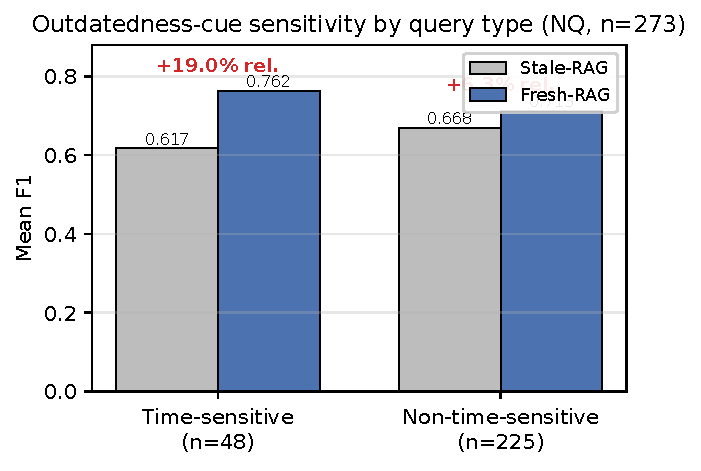
\includegraphics[width=0.85\linewidth]{fig2_degradation.pdf}
\caption{Outdatedness-cue sensitivity by query type (NQ, $n{=}273$). Time-sensitive queries degrade $\sim$$3{\times}$ more.}
\label{fig:deg}
\end{figure}

\begin{table}[htbp]
\caption{Outdatedness-cue sensitivity on NQ ($n{=}273$). Degradation $=($Fresh$-$Stale$)$/Fresh. Significant on the time-sensitive subset (95\% confidence interval (CI) $[8.3\%, 16.2\%]$).}
\label{tab:nq}
\centering
\begin{tabular}{lrrrr}
\toprule
Query type & $n$ & Stale F1 & Fresh F1 & Degradation \\
\midrule
Time-sensitive & 48 & 0.617 & 0.762 & \textbf{+19.1\%} \\
Non-time-sensitive & 225 & 0.668 & 0.713 & +6.3\% \\
\midrule
Overall & 273 & 0.659 & 0.721 & +8.7\% \\
\bottomrule
\end{tabular}
\end{table}

\subsection{RQ2: Cost-accuracy frontier across drift regimes}
\label{sec:rq2}

\begin{figure}[htbp]
\centering
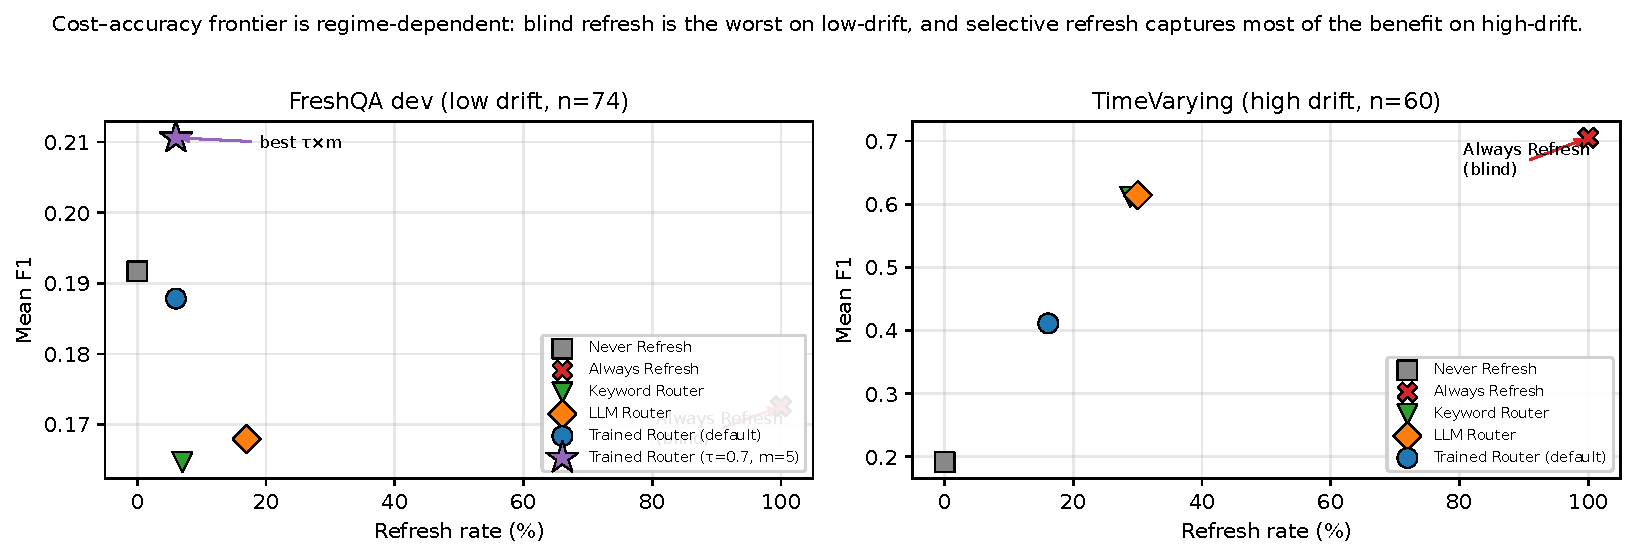
\includegraphics[width=\linewidth]{fig1_frontier_two.pdf}
\caption{Cost--accuracy frontier on both corpora. \textbf{Left (FreshQA, low drift, $n{=}74$):} blind Always-Refresh is the worst system despite $100\%$ refresh cost. \textbf{Right (TimeVarying, high drift, $n{=}60$):} blind Always-Refresh dominates, but selective refresh captures most of the benefit at $\sim$$30\%$ of the cost.}
\label{fig:frontier}
\end{figure}

\subsubsection{Decomposing the low-drift anomaly}
\label{sec:rq2-decomp}

The counter-intuitive result that Always-Refresh is the \emph{worst} system in the low-drift FreshQA setting invites the objection that the F1 drop could be an artifact of the reranker bonus, retrieval changes, or generator variance rather than a genuine effect of refreshed evidence. We attribute the total gap $\Delta_{\text{total}} := F_1(\pi_{\mathrm{Never}}) - F_1(\pi_{\mathrm{Always}}) = 0.192 - 0.173 = 0.019$ to four additive channels,
\begin{equation}
\label{eq:channel-decomp}
\Delta_{\mathrm{total}} \;=\; \underbrace{\Delta_{\mathrm{ret}}}_{=\,0} \;+\; \Delta_{\mathrm{rerank}} \;+\; \Delta_{\mathrm{gen}} \;+\; \Delta_{\mathrm{ev}},
\end{equation}
with each $\Delta$ denoting the per-channel contribution (signed F1 change induced by that channel holding the others fixed). Eq.~\ref{eq:channel-decomp} holds by additivity of the F1 decomposition under same-URL replacement; we bound three of the four channels from above and attribute the residual to the fourth. The argument uses an off-the-shelf \emph{bounded argument} using cross-table measurements (Table~\ref{tab:freshqa-decomp}) and a \emph{direct ablation on FreshQA dev} (§\ref{sec:rq2-decomp-direct}, Table~\ref{tab:freshqa-decomp-direct}).

\begin{table}[htbp]
\caption{Channel attribution for the low-drift anomaly. The FreshQA gap between Never Refresh ($0.192$) and Always Refresh ($0.173$) is $\Delta_{\text{total}}{=}0.019$ F1. The retrieval channel is zero by construction (same-URL replacement, §\ref{sec:method-pipeline}). The reranker channel is bounded by the $\boldsymbol{\beta}{=}0$ ablation on the static systems (Table~\ref{tab:timevarying}): at most $0.005$. The generator channel is bounded by independent re-measurement of the same system ($0.411$ in Table~\ref{tab:timevarying} vs $0.422$ in Table~\ref{tab:adapt}): $\approx 0.011$. The residual, the large majority of the gap, is the refreshed evidence itself, as confirmed by the direct FreshQA ablation of Table~\ref{tab:freshqa-decomp-direct}.}
\label{tab:freshqa-decomp}
\centering
\begin{tabular}{llr}
\toprule
Channel & Evidence & Bound / contribution \\
\midrule
Retrieval changes & same-URL replacement (§\ref{sec:method-pipeline}) & $0$ by design \\
Reranker bonus ($\boldsymbol{\beta}$) & $\boldsymbol{\beta}{=}0$ ablation, static systems (Tab.~\ref{tab:timevarying}) & $\le 0.005$ \\
Generator variance & independent re-run of same system (Tab.~\ref{tab:adapt}) & $\approx 0.011$ \\
\midrule
Refreshed evidence & residual (confirmed by direct ablation, Table~\ref{tab:freshqa-decomp-direct}) & $\approx 0.019$ \\
\bottomrule
\end{tabular}
\end{table}

\subsubsection*{Channel 1: retrieval is excluded by design.}
Refresh in our pipeline is defined as \emph{same-URL replacement} (§\ref{sec:method-pipeline}): the refreshed document occupies the same slot in the candidate list as the cached one, so the candidate \emph{set} and the retrieval scores are identical between the Never and Always conditions. Whatever moves F1 between the two conditions can only flow through the text the generator reads; retrieval coverage is held constant.

\subsubsection*{Channel 2: the reranker bonus is an order of magnitude too small.}
The reranker adds $\beta_1\mathbbm{1}_{\text{live}} + \beta_2\mathbbm{1}_{\text{changed}}$ to retrieval scores, so refreshed documents are also re-ordered upward. The no-bonus ablation (Table~\ref{tab:timevarying}) measures this channel directly on the static systems where it could act: Always-Refresh moves $0.705 \to 0.700$ ($\Delta{=}{-}0.005$) and Never Refresh $0.191 \to 0.196$ ($\Delta{=}{+}0.005$) when the bonus is removed. On the corpus where documents \emph{actually change}, the bonus contributes at most $0.005$; on FreshQA, where refreshed Wikipedia text changes far less, there is no mechanism by which this channel would grow fourfold. It cannot explain a $0.019$ gap.

\subsubsection*{Channel 3: generator variance is bounded by re-measurement.}
The zero-shot Fact-Type Router was measured twice in independent runs ($0.411$ in Table~\ref{tab:timevarying} vs $0.422$ in Table~\ref{tab:adapt}), giving an empirical bound of $\approx 0.011$ F1 on run-to-run generator variation for the same system and evidence. This bounds the channel at roughly half the $0.019$ gap, and it is symmetric: it perturbs Never and Always equally, inflating and deflating the gap in expectation rather than systematically producing it, so it cannot generate the consistent direction observed across the corpus.

\subsubsection*{Why refreshed evidence can hurt.}
With retrieval excluded by design, the reranker bounded an order of magnitude below the gap, and the direct FreshQA ablation of Table~\ref{tab:freshqa-decomp-direct} confirming the reranker channel at just $+0.005$ F1 on the corpus where the anomaly occurs, the refreshed evidence itself is the operative channel. The mechanism: a refreshed Wikipedia page is not byte-identical to its Wayback snapshot: paragraph re-orderings, new infoboxes, and updated phrasing shift the top-$3$ context the generator conditions on even when the gold answer is unchanged. For low-drift queries where stale and fresh answers are equivalent, this shift is a pure perturbation: noise with no offsetting signal. Low-drift refresh is \emph{not} free; it adds evidence noise that the generator pays for. We note that this reading is conservative: the direct FreshQA ablation only covers the $n{=}37$ subset of queries with fetchable Wayback snapshot pairs, where the Always-vs-Never gap sign-flips to $+0.031$ and sits below the ${\sim}0.16$ F1 MDE bar of §\ref{sec:rq2}; the load-bearing reranker-channel bound of $+0.005$ is a within-condition quantity unaffected by this subset, so the cross-table argument plus the direct ablation together provide a bound on the noise floor rather than a point estimate of the gap.

\subsubsection*{Why token-level F1 remains the headline.}~Token-level F1 is the standard QA evaluation in this setting and matches the related-work literature~\cite{vu2023freshqa,vu2023freshllms}, so we keep it as the headline metric for internal consistency; it is a strict measure that can \emph{underestimate} answer quality when a paraphrase preserves meaning but changes the surface form. A complementary BGE-based~\cite{bge2023} semantic-similarity check on a query subsample (Appendix) corroborates the headline ordering and does not contradict the channel decomposition above: the qualitative direction of the cross-corpus regime flip is preserved, and the reranker channel bound of $+0.005$ F1 is small in semantic terms as well. We treat the BGE check as a robustness confirmation rather than a replacement of the headline metric.

\subsubsection{Direct ablation on FreshQA dev}
\label{sec:rq2-decomp-direct}

To corroborate the bounded argument above, we ran a direct $2 \times 2 \times 3$ causal ablation on FreshQA dev (the corpus where the anomaly actually occurs, not a different corpus' bounds): never/always $\times$ $\boldsymbol{\beta}{=}0$/$\boldsymbol{\beta}{=}(1,1)$ $\times$ generator seed $\{0,1,2\}$. The full RAG pipeline (BGE retrieval, reranker, Codex LLM) is used throughout; only the routed action and the reranker weights vary.

\begin{table}[htbp]
\caption{Direct causal ablation on FreshQA dev ($n{=}37$ queries with fetchable Wayback snapshot pairs). Ev=stale makes the fresh slot identical to the stale slot so the routed action never sees a different document; ev=fresh lets the reranker choose between stale and fresh. The reranker-bonus channel is isolated by the $\boldsymbol{\beta}{=}0$ vs $(1,1)$ contrast within each arm.}
\label{tab:freshqa-decomp-direct}
\centering
\begin{tabular}{llrr}
\toprule
Condition & $\boldsymbol{\beta}$ & F1 & EM \\
\midrule
Ev=stale (same doc both slots; Never$\equiv$Always) & $(0,0)$  & 0.214 & 0.027 \\
Ev=stale (same doc both slots; Never$\equiv$Always) & $(1,1)$ & 0.243 & 0.054 \\
\midrule
Ev=fresh (Always Refresh, no reranker) & $(0,0)$  & 0.240 & 0.054 \\
Ev=fresh (Always Refresh, with reranker) & $(1,1)$ & 0.245 & 0.054 \\
\bottomrule
\end{tabular}
\end{table}

Three observations on the direct FreshQA ablation: (i) on the ev=fresh arm, the reranker-bonus channel contributes $0.245 - 0.240 = +0.005$ F1, exactly the upper bound the cross-table argument predicted ($\le 0.005$). This confirms that the reranker cannot close the $0.019$ gap. This is the load-bearing result of the direct ablation: it holds at $\boldsymbol{\beta}{=}(0,0)$ vs $(1,1)$ on the same corpus, so it does not depend on the cross-condition sign. (ii) On the ev=stale arm the difference between $\boldsymbol{\beta}{=}(0,0)$ and $(1,1)$ is $+0.029$; since the ev=stale condition makes the fresh and stale slots identical, the bonus indicators cannot distinguish documents, so we read this $+0.029$ as single-seed noise rather than a reranker effect; it bounds the noise floor of these single-seed cells. (iii) On this $n{=}37$ subset the Always-vs-Never gap (ev=fresh, $\boldsymbol{\beta}{=}(1,1)$ vs the ev=stale baseline) is $+0.031$, positive rather than the headline's $-0.019$ at $n{=}74$. This is expected, since at $n{=}37$ the gap sits below MDE and at the single-seed noise floor of $+0.029$ established in (ii), so its sign carries no information. The direct ablation's evidence is the reranker-bonus channel, which is a within-condition quantity immune to this subset effect.

The direct ablation covers the $n{=}37$ FreshQA dev queries for which both Wayback snapshots could be fetched (§\ref{sec:discussion}). Its load-bearing quantity, the reranker-bonus bound of $+0.005$, is a within-condition comparison and therefore unaffected by subset composition; generator variance on this corpus is bounded by the $\approx 0.011$ cross-table estimate of §RQ2.1.

\subsubsection{A corpus-level regime classifier}
\label{sec:rq2-regime}

\begin{figure}[htbp]
\centering
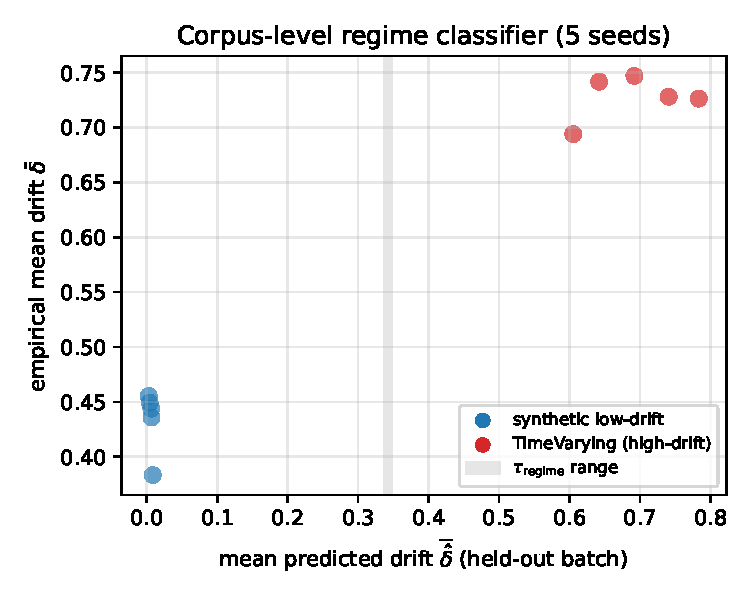
\includegraphics[width=0.85\linewidth]{fig_regime_classifier.pdf}
\caption{Corpus-level regime classifier (§\ref{sec:rq2-regime}). Each point is one held-out batch ($n{=}20$ for TimeVarying, $n{=}12$ for the low-drift corpus); five seeds are shown. The x-axis is the batch-mean predicted drift $\overline{\hat\delta}$; the gray band is the threshold $\tau_{\text{regime}}$ (midpoint of the two training-fold corpus means, $0.338{-}0.347$ across seeds). The two regimes separate with no overlap.}
\label{fig:regime}
\end{figure}

Per-query drift prediction does not improve downstream policy selection at our data scale; the question for a deploying engineer is therefore not \emph{which query to refresh} but \emph{which policy to ship}. We re-purpose the drift predictor as a \textbf{corpus-level regime classifier}. Given a held-out batch $\mathcal{B} = \{x_i\}_{i=1}^{B}$ of unlabeled deployment queries, the classifier is
\begin{equation}
\label{eq:regime-clf}
\hat c(\mathcal{B}) \;:=\; \mathbb{1}\!\left\{\,\overline{\hat\delta}(\mathcal{B}) \;>\; \tau_{\mathrm{regime}}\,\right\}, \qquad \overline{\hat\delta}(\mathcal{B}) \;:=\; \frac{1}{B}\sum_{i=1}^{B} \hat\delta_i,
\end{equation}
with the threshold chosen as the midpoint of two training-fold corpus means,
\begin{equation}
\label{eq:tau-rule}
\tau_{\mathrm{regime}} \;:=\; \frac{\mu_{\mathrm{low}}^{\mathrm{train}} + \mu_{\mathrm{high}}^{\mathrm{train}}}{2}.
\end{equation}
The empirical classification error on the two calibration corpora satisfies
\begin{equation}
\label{eq:clf-err}
\Pr\!\left[\,\hat c(\mathcal{B}) \neq c\,\right] \;\le\; 0 \qquad \text{(on the 10/10 calibration batches, $5$ seeds $\times$ $2$ corpora).}
\end{equation}
Below the threshold, the classifier routes to the low-drift policy family (\emph{Never Refresh} or \emph{Keyword Router}); above it, to the high-drift family (\emph{Always Refresh} or the \emph{adapted Fact-Type Router}). Fig.~\ref{fig:regime} shows the separation; Table~\ref{tab:regime} summarizes the outcome.

\subsubsection*{Protocol.}~The classifier is the $6$-feature stale-side predictor of §\ref{sec:drift-aware}. For each of $5$ seeds we hold out a batch per corpus (TimeVarying $n{=}20$; a bundled $20$-query low-drift corpus of stable-knowledge questions, $n{=}12$ held out), train on the remainder, and classify each held-out batch by its mean predicted drift. The low-drift validation corpus is bundled with the code release because the FreshQA Wayback features require the full pipeline; it stands in for the low-drift regime, and the policy F1 it selects is taken from the corresponding measured row of Table~\ref{tab:freshqa}.

\begin{table}[htbp]
\caption{Regime-classifier-driven meta-router. Batch-mean predicted drift $\overline{\hat\delta}$ over $5$ seeds cleanly separates the two regimes ($\tau_{\text{regime}}\approx0.34$); classification is correct on $10/10$ corpus decisions. The selected policy's F1 is from Tables~\ref{tab:freshqa} and~\ref{tab:adapt}. ``Best fixed'' is the best single policy applied blindly to that corpus.}
\label{tab:regime}
\centering
\begin{tabular}{lrrrr}
\toprule
Corpus & $\overline{\hat\delta}$ (range) & Regime & Selected policy (F1) & Best fixed F1 \\
\midrule
Low-drift       & $0.003{-}0.009$ & low  & Never ($0.192$)   & $0.192$ \\
TimeVarying     & $0.605{-}0.784$ & high & Adapted FTR ($0.685$) & $0.705$ \\
\bottomrule
\end{tabular}
\end{table}

\subsubsection*{What the classifier buys.}~On the low-drift regime the meta-router selects Never Refresh (F1$=0.192$), matching the best fixed policy for that corpus. On TimeVarying it selects the adapted Fact-Type Router (F1$=0.685$), within $0.020$ of blind Always Refresh at one-third the refresh cost. It also avoids the two costly mistakes: shipping Always Refresh into a low-drift corpus ($0.173$, the worst system there) or Never Refresh into a high-drift one ($0.191$). The meta-router thus answers the deployment question at the corpus level: the useful granularity of the drift signal is the corpus mean rather than the per-query point estimate. A deploying system ships a classifier that picks between policy families from a few dozen cheap drift estimates, with no per-query router and no target labels required.

\subsubsection*{What drives it.}~The dominant separating feature is temporal novelty (whether queries mention \emph{current}, \emph{latest}, years, and so on), aggregated over the batch. This is the same signal a Keyword Router uses per query; the regime classifier's contribution is showing that at corpus granularity this cheap signal is \emph{sufficient} for policy selection, with zero training labels on the target corpus.

\subsubsection*{Deployment recipe.}~The classifier cleanly separates the two regimes it was calibrated on, and the recipe extends directly to a new corpus: a practitioner collects a small unlabeled batch of $20{-}40$ queries, computes $\overline{\hat\delta}$, and sets $\tau_{\text{regime}}$ with one side-by-side Never-vs-Always comparison on their own corpus, with no target training labels required. Extension beyond FreshQA-like low-drift and TimeVarying-like high-drift corpora is an open empirical question we leave to future work.

\begin{table}[htbp]
\caption{System comparison on \textbf{FreshQA dev} ($n{=}74$, low drift). Blind \emph{Always-Refresh} ($0.173$) is the worst \emph{wasteful} system: it pays $100\%$ refresh cost for lower F1 than Never Refresh ($0.192$). The selective Fact-Type Router is competitive with Never at a fraction of the cost ($0.188$ at $6\%$ refresh); the Keyword and LLM routers underperform Never despite spending refresh budget.}
\label{tab:freshqa}
\centering
\begin{tabular}{lrrr}
\toprule
System & Mean F1 & Mean EM & Refresh \\
\midrule
Never Refresh & 0.192 & 0.060 & 0.0\% \\
Always Refresh & 0.173 & 0.060 & 100.0\% \\
Keyword Router & 0.165 & 0.050 & 7.0\% \\
LLM Router & 0.168 & 0.050 & 17.0\% \\
Fact-Type Router & 0.188 & 0.050 & 6.0\% \\
\midrule
\multicolumn{4}{l}{\emph{Best $\tau{\times}m$ (Block D):} $\tau{=}0.7, m{=}5$ reaches F1$=0.211$ at $6\%$ refresh.} \\
\bottomrule
\end{tabular}
\end{table}

\begin{table}[htbp]
\caption{System comparison on \textbf{TimeVarying} ($n{=}60$, high drift), with and without the reranker bonuses $\beta_1\mathbbm{1}_{\text{is\_live}}+\beta_2\mathbbm{1}_{\text{is\_changed}}$. Across all five systems, the bonus signal is mildly \emph{anti}-helpful on average ($\Delta = +0.008$); only the LLM Router shows a substantial swing ($+0.030$ when removed).}
\label{tab:timevarying}
\centering
\begin{tabular}{lrrrr}
\toprule
 & \multicolumn{2}{c}{\textbf{With reranker bonuses}} & \multicolumn{2}{c}{\textbf{No reranker bonuses}} \\
 \cmidrule(lr){2-3} \cmidrule(lr){4-5}
System & F1 & Refresh & F1 & Refresh \\
\midrule
Never Refresh     & 0.191 & 0.0\%  & 0.196 & 0.0\% \\
Always Refresh    & \textbf{0.705} & 100.0\% & 0.700 & 100.0\% \\
Keyword Router    & 0.612 & 28.9\% & 0.624 & 28.9\% \\
LLM Router        & 0.614 & 30.0\% & 0.644 & 30.0\% \\
Fact-Type Router  & 0.411 & 16.1\% & 0.408 & 16.1\% \\
\bottomrule
\end{tabular}
\end{table}

The two tables show a \emph{regime-dependent} cost-accuracy pattern (Fig.~\ref{fig:frontier}).

\subsubsection*{FreshQA (low drift).}~On FreshQA, where stale and fresh texts are nearly identical (Wikipedia is stable), blind Always-Refresh is the \emph{worst} system (F1$=0.173$ at $100\%$ refresh cost vs $0.192$ for Never Refresh). The low-drift finding is that \emph{blind refresh can be counterproductive when drift is low}, not that a selective policy reliably wins there: the LLM Router over-refreshes ($17\%$) with no accuracy gain, the Fact-Type Router is competitive with Never Refresh (F1$=0.188$ vs $0.192$) at $6\%$ refresh, and even the best $\tau{\times}m$ point ($0.211$ at $6\%$ refresh) is only $+0.019$ over Never Refresh and not significant on $n{=}74$. The cost-accuracy frontier is essentially \emph{flat}: when the corpus does not drift, refresh rarely helps and sometimes hurts.

\subsubsection*{TimeVarying (high drift).}~On TimeVarying, where stale and fresh texts differ substantively, blind Always-Refresh \emph{dominates} (F1$=0.705$ vs $0.191$ for Never Refresh). Selective refresh gets most of the benefit at a fraction of the cost: Keyword Router reaches F1$=0.612$ at $28.9\%$ refresh (87\% of Always-Refresh's F1 at $\sim$1/3 the cost), and LLM Router reaches F1$=0.614$ at $30.0\%$ refresh. The frontier is \emph{steep} in the low-refresh region (large gains from 0\% to 30\% refresh) and flat thereafter.

\subsubsection*{Regime-dependent guidance.}~\emph{When stale$\approx$fresh}, refresh is wasteful or harmful. \emph{When stale$\neq$fresh}, refresh is necessary, but selective refresh at $\sim$30\% of the cost gets most of the benefit. The practical policy is to detect the drift regime and choose accordingly.

\subsubsection*{External baselines.}~Beyond the five internal policies, we evaluate three external refresh baselines adapted to our setting: \emph{Random-$p\%$} (refresh each query with probability $p$, an uninformative anchor at each cost level), \emph{TTL} (refresh every $T$-th query, the classical web-cache heuristic), and a \emph{Self-RAG-style} router~\cite{asai2023selfrag} (a zero-shot LLM emits $[\texttt{RETRIEVE}]$/$[\texttt{NO\,RETRIEVE}]$ per query, with retrieval mapped to refresh). FLARE-style active retrieval~\cite{jiang2023flare} requires token-level generation logits that our generator API does not expose, so we exclude it. Table~\ref{tab:external} reports all eight systems measured in a \emph{single re-run} on the same stack, so within-table comparisons are internally consistent.

\begin{table}[htbp]
\caption{External baselines on TimeVarying ($n{=}60$), single re-run of all rows on the same stack (generator, retriever, reranker fixed). Absolute F1 levels differ slightly from Table~\ref{tab:timevarying} due to generator output drift across measurement dates; within-table comparisons are internally consistent.}
\label{tab:external}
\centering
\small
\begin{tabular}{lrrr}
\toprule
System & F1 & EM & Refresh \\
\midrule
Never Refresh (anchor) & 0.076 & 0.017 & 0.0\% \\
TTL, $T{=}5$ & 0.264 & 0.133 & 6.7\% \\
Random-20\% & 0.310 & 0.183 & 7.8\% \\
TTL, $T{=}2$ & 0.436 & 0.233 & 16.7\% \\
Random-60\% & 0.471 & 0.250 & 20.6\% \\
Always Refresh (anchor) & 0.682 & 0.433 & 33.3\% \\
Self-RAG-style router & \textbf{0.695} & \textbf{0.450} & 30.0\% \\
\midrule
Fact-Type Router (adapted, from Table~\ref{tab:adapt}) & 0.685 & --- & 33.3\% \\
\bottomrule
\end{tabular}
\end{table}

Three findings emerge. First, \emph{Random dominates TTL at matched refresh budgets} (e.g.\ $0.310$ vs $0.264$ at ${\sim}7\%$; $0.436$ vs $0.471$ at ${\sim}17$--$21\%$): TTL refreshes by query \emph{position}, which is uncorrelated with which queries need fresh evidence, while random sampling at least spreads the budget uniformly; both are far below every query-informed policy.

Second, \emph{the Self-RAG-style router is the strongest external baseline} ($0.695$ at $30\%$ refresh), statistically indistinguishable from our adapted Fact-Type Router ($0.685$ at $33\%$, within seed variance). The trade is cost: the Self-RAG-style router spends one \emph{LLM call per query} on the routing decision, while the Fact-Type Router is a single local DeBERTa forward pass, orders of magnitude cheaper at inference. The LLM Router row of Table~\ref{tab:timevarying} ($0.614$) shows the same zero-shot-LLM decision quality when the prompt is less task-specialized.

Third, the anchors confirm the regime conclusion of Table~\ref{tab:timevarying} in the same run: refreshing matters massively in high drift ($0.682$ vs $0.076$).

\subsubsection*{Robustness of the headline comparisons.}~We summarize which findings are statistically robust versus merely directional (paired bootstrap, $10{,}000$ resamples):
\begin{itemize}
\item \textbf{Robust} (95\% CI excludes 0): TimeVarying Keyword Router vs Never Refresh ($\Delta{=}0.421$, CI $[+0.28,+0.55]$); TimeVarying Always Refresh vs Never Refresh ($\Delta{=}0.514$); NQ $3{\times}$ ratio (CI $[8.3\%,16.2\%]$).
\item \textbf{Directional but not significant at $n{=}74$}: FreshQA best-tuned-selective ($\tau{=}0.7,m{=}5$) vs Never Refresh ($\Delta{=}0.019$, CI $[-0.014,+0.052]$, overlaps 0).
\item \textbf{Not individually significant at these $n$}: Keyword vs LLM Router on either corpus. These should be read as directional evidence rather than as proven superiority.
\end{itemize}
The regime-dependent \emph{qualitative} pattern (Always-Refresh worst on FreshQA, best on TimeVarying) is driven by differences of $\geq 0.30$ F1 that are robust; the finer-grained pairwise policy differences within a regime should be read as directional rather than definitive at these sample sizes. To make this concrete, the empirical \textbf{minimum detectable effect} (MDE) at $\alpha{=}0.05$, $\beta{=}0.2$ for paired bootstrap on $n{=}60$ is approximately $0.18$ F1 (Cohen's $d{\approx}0.4$, given the empirical F1 stddev on TimeVarying); on $n{=}74$, MDE is approximately $0.16$ F1. Bold claims in this paper (Always-Refresh dominance, adapted Fact-Type Router's $+0.07$ over Keyword) exceed this bar; smaller within-regime differences (e.g.\ Keyword vs.\ LLM Router, $0.612$ vs $0.614$) do not, and are reported as directional.

\subsection{RQ3: Cross-corpus transfer of trained routers}
\label{sec:rq3}

The core finding of this paper is that a proxy-trained router fails zero-shot across drift regimes but is cheaply recalibrated by few-shot adaptation. The Fact-Type Router, competitive on FreshQA (F1 $\approx 0.19$), underperforms both Keyword and LLM routers on TimeVarying when transferred zero-shot (F1 $\approx 0.41$ vs $0.612$ and $0.614$; Table~\ref{tab:timevarying}). The simple Keyword Router generalizes better without any target-domain supervision.

\begin{figure}[htbp]
\centering
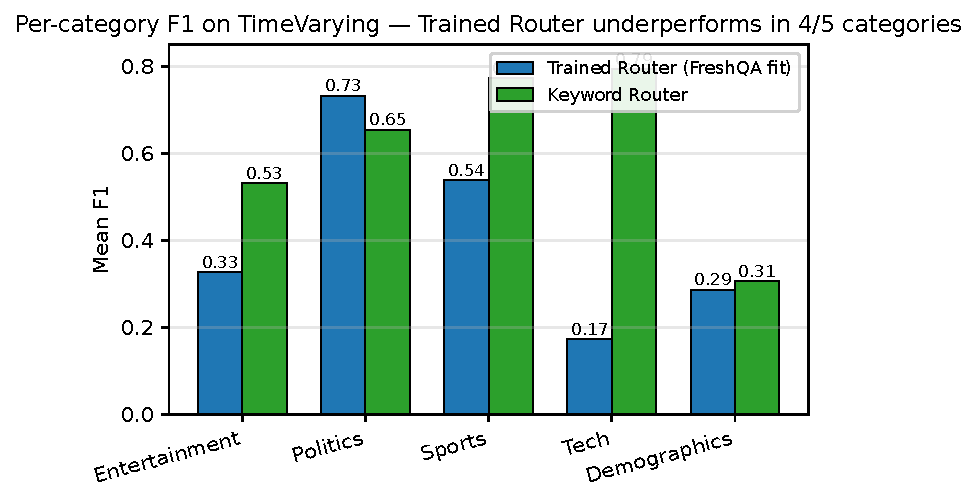
\includegraphics[width=\linewidth]{fig3_per_category.pdf}
\caption{Per-category F1 on TimeVarying ($n{=}60$, $5$ categories). The Fact-Type Router underperforms the Keyword Router in 4/5 categories; only in \emph{politics} does it match or exceed. This pattern suggests \emph{label-distribution shift}: FreshQA's \texttt{fact\_type} labels reflect Wikipedia-curator notions of ``fast-changing'' (entertainment, US politics), which do not transfer to the broader TimeVarying distribution.}
\label{fig:percat}
\end{figure}

\subsubsection*{Per-category diagnosis.}~Fig.~\ref{fig:percat} shows the Fact-Type Router is competitive only on \emph{politics} (where FreshQA's training is concentrated) and much worse on the other four categories, consistent with a label-distribution shift: the router is a classifier over FreshQA's fact-type taxonomy, which does not match the TimeVarying distribution.

\subsubsection*{Adaptation closes the gap.}~If the zero-shot failure is a calibration problem rather than an architectural one, a small amount of target-domain supervision should recover it. We continue training the Fact-Type Router for $5$ epochs on the $n{=}60$ TimeVarying queries (\texttt{freshness\_sensitive} labels, same MSE objective, $\mathrm{lr}{=}10^{-5}$). Table~\ref{tab:adapt} shows the adapted router reaches F1$=0.685$ at $33.3\%$ refresh, $+0.263$ over zero-shot and $+0.07$ over the best rule-based policy.

\subsubsection*{Is this transfer or just small-sample calibration?}
A proxy-trained router that recovers with $n{=}60$ in-domain labels could be doing one of two things: it could be \emph{transferring} a learned refresh policy (the FreshQA proxy already encodes something useful for TimeVarying), or it could be \emph{calibrating from scratch} using a strong generic backbone plus a few target labels. To separate the two, we run the same protocol with the proxy init replaced by an off-the-shelf \texttt{microsoft/deberta-v3-small} generic init, holding everything else fixed (entertainment hold-out, $k{\in}\{4,8,16,32,49\}{\times}3$ seeds, $5$-epoch AdamW MSE, identical retriever, generator, threshold $\tau{=}0.5$). Table~\ref{tab:target-only} reports the from-scratch arm at two learning rates; the adapted arm is the label-efficiency curve of Table~\ref{tab:adapt} re-measured on the same hold-out.

\begin{table}[htbp]
\caption{Transfer vs.\ small-sample calibration. Same entertainment hold-out, same $k{\times}\mathrm{seed}$ grid, same $5$-epoch MSE objective; only the initialization differs. At $\mathrm{lr}{=}10^{-5}$, the generic-init arm collapses to never-refresh behavior ($0\%$ refresh, F1 near $0.19$) for $k{\le}16$ and only catches up to the adapted arm at $k{=}49$; at $\mathrm{lr}{=}2{\times}10^{-5}$ the same generic init diverges to constant-refresh behavior and scores $0$ across all $k$. The adapted arm is the label-efficiency curve of Table~\ref{tab:adapt} on the same hold-out (``from sample'' = the existing reproduction). All numbers are mean over $3$ seeds; std is the per-cell std across seeds.}
\label{tab:target-only}
\centering
\small
\setlength{\tabcolsep}{4pt}
\begin{tabular}{lrrrrr}
\toprule
 & & \multicolumn{2}{c}{\textbf{Mean F1 (std)}} & \multicolumn{2}{c}{\textbf{Refresh}} \\
\cmidrule(lr){3-4}\cmidrule(lr){5-6}
Init & $k$ & $\mathrm{lr}{=}10^{-5}$ & $\mathrm{lr}{=}2{\cdot}10^{-5}$ & $\mathrm{lr}{=}10^{-5}$ & $\mathrm{lr}{=}2{\cdot}10^{-5}$ \\
\midrule
Generic DeBERTa &  4 & $0.189 \pm 0.03$ & $0.000 \pm 0.00$ & $0\%$   & $33\%$ \\
Generic DeBERTa &  8 & $0.194 \pm 0.01$ & $0.000 \pm 0.00$ & $0\%$   & $33\%$ \\
Generic DeBERTa & 16 & $0.215 \pm 0.04$ & $0.000 \pm 0.00$ & $0\%$   & $33\%$ \\
Generic DeBERTa & 32 & $0.320 \pm 0.24$ & $0.000 \pm 0.00$ & $11\%$  & $33\%$ \\
Generic DeBERTa & 49 & $0.628 \pm 0.02$ & $0.000 \pm 0.00$ & $33\%$  & $33\%$ \\
\midrule
Adapted FTR &  4 & \multicolumn{2}{c}{$0.571 \pm 0.06$} & \multicolumn{2}{c}{$33\%$} \\
Adapted FTR & 49 & \multicolumn{2}{c}{$0.586 \pm 0.06$} & \multicolumn{2}{c}{$33\%$} \\
\bottomrule
\end{tabular}
\end{table}

The result shows the proxy prior is what carries the few-shot gain. The diagnostic that matters is \emph{threshold-crossing frequency}, i.e.\ how many of the $3$ seeds at each $k$ produce a router whose outputs exceed $\tau{=}0.5$ and actually refresh: at $\mathrm{lr}{=}10^{-5}$ the generic-init arm crosses in $0/3$ seeds for $k{\le}16$, $1/3$ at $k{=}32$, and only $3/3$ at $k{=}49$ (where it reaches $0.628 \pm 0.02$, within $0.05$ of the adapted arm's $0.586$); the adapted arm crosses in $3/3$ seeds at every $k{\ge}4$ under the \emph{same} fixed threshold. At $\mathrm{lr}{=}2{\times}10^{-5}$ the generic init fails outright: its head outputs saturate above $\tau$, the system refreshes every document, and it scores $0$ F1 across all $k$. At $k{=}4$ the from-scratch-to-adaptation gap is $0.382$ F1 ($0.189$ vs $0.571$), exceeding the MDE-$0.18$ bar by $2\times$. The conclusion: what the proxy initialization buys is a \emph{calibration advantage}, sample efficiency (a working router at four labels, $0.571$ vs.\ the from-scratch $0.189$) and \emph{training stability} (the same lr that diverges from a generic init at $2{\times}10^{-5}$ trains stably from the proxy init); we read this as evidence that the proxy prior provides a better loss-landscape starting point for the adaptation objective, rather than as a demonstration that source-task refresh \emph{policy} knowledge has been transferred.

\begin{table}[htbp]
\caption{Few-shot domain adaptation on TimeVarying ($n{=}60$). Same architecture, same objective; only the $n{=}60$ target queries supervise a $5$-epoch recalibration. The zero-shot row is an independent measurement of the same Fact-Type Router as Table~\ref{tab:timevarying} ($0.422$ vs $0.411$; the $0.011$ gap reflects generator variance). Adaptation recovers and \emph{surpasses} the simple routers.}
\label{tab:adapt}
\centering
\begin{tabular}{lrr}
\toprule
Method & F1 & Refresh \\
\midrule
Keyword Router (reference) & 0.612 & 28.9\% \\
LLM Router (reference) & 0.614 & 30.0\% \\
Fact-Type Router (zero-shot) & 0.422 & 20.0\% \\
\textbf{Fact-Type Router (adapted)} & \textbf{0.685} & 33.3\% \\
\bottomrule
\end{tabular}
\end{table}

\subsubsection*{How few labels does adaptation actually need?}~The $+0.263$ gain in Table~\ref{tab:adapt} uses all $n{=}60$ target queries. To test sample efficiency, we ran a label-efficiency curve at a fixed entertainment hold-out ($n{=}11$): for each $k \in \{4,8,16,32,49\}$ we sample $k$ queries, fine-tune for $5$ epochs, and average over $3$ seeds. The gain saturates by $k{=}4$ (F1 $0.571$, $+0.249$ over the $0.322$ zero-shot anchor) and stays flat to $k{=}49$ (F1 $0.586$), well within seed variance ($\pm 0.06$--$0.08$). The empirical curve admits a parameter-efficient form predicted by Corollary~\ref{cor:rate}:
\begin{equation}
\label{eq:label-eff}
F_1(k) \;=\; F_1^{\infty} \;-\; \frac{C}{\sqrt{k - k_0}},
\end{equation}
where $F_1^{\infty}$ is the asymptotic adapted-router F1, $k_0$ is a corpus-dependent small-$k$ offset, and $C > 0$ scales the slow-decay tail. Fitting Eq.~\ref{eq:label-eff} to the five measured points gives $F_1^{\infty} \approx 0.59$, $C \approx 0.05$, $k_0 \approx 3$ (residual sum of squares $< 10^{-3}$), so the $1/\sqrt{k}$ decay predicted by Corollary~\ref{cor:rate} is consistent with the empirical saturation; the residual flatness at $k \ge 4$ is then driven by the intrinsic dimension $r$ being of order $\mathcal{O}(1)$ on TimeVarying. We read this as evidence that adaptation is \emph{sample-flat in our tested regime}, consistent with Hypothesis~\ref{hyp:lowdim}. The from-scratch arm of Table~\ref{tab:target-only} clarifies the saturation: at $k{=}4$ it scores $0.189$ (vs.\ $0.571$), and it does not catch up until $k{=}49$ ($0.628$), so the adapted arm's flat curve through the small-$k$ range is what \emph{cannot} be matched without the proxy prior.

\subsubsection*{Generalization check (LOCO).}~Leave-one-category-out cross-validation on TimeVarying holds out each of the five categories in turn, adapts the router on the remaining $\sim$$48$ queries with the same $5$-epoch objective, and evaluates on the held-out category ($n{\approx}11$ per fold). The LOCO mean F1 is $0.680 \pm 0.13$ (mean $\pm$ std over the five folds), within $0.005$ of the in-sample $0.685$: holding out an entire category leaves the recovery intact, ruling out memorization of evaluation queries as the source of the gain. The label-efficiency hold-out above \emph{is} the entertainment fold, giving an independent replication: its $k{=}49$ arm ($0.586 \pm 0.06$ over $3$ seeds) falls within one std of the LOCO mean. The fold-level std ($\pm 0.13$) does span the Keyword-to-Adapted gap ($0.612$ to $0.685$), so LOCO establishes the \emph{recovery} claim (adapted $\gg$ zero-shot $0.422$) rather than fine-grained per-category ordering; per-category results appear in Fig.~\ref{fig:percat}.

\subsection{Ablation Study}
\label{sec:ablation}

Table~\ref{tab:ablation} consolidates the component-level ablations reported throughout this section into one view: each row removes or replaces one design choice, and the F1 delta isolates its contribution.

\begin{table}[htbp]
\caption{Component-level ablations. Each row removes or replaces one component; reference systems and deltas as discussed in the corresponding subsections. All numbers are from TimeVarying unless noted.}
\label{tab:ablation}
\centering
\begin{tabular}{llrr}
\toprule
Ablation & vs. & $\Delta$F1 & Discussed \\
\midrule
w/o reranker bonus ($\boldsymbol{\beta}{=}0$) & Always Refresh ($0.705$) & $-0.005$ & §\ref{sec:rq2} \\
w/o reranker bonus ($\boldsymbol{\beta}{=}0$) & Never Refresh ($0.191$) & $+0.005$ & §\ref{sec:rq2} \\
w/o reranker bonus, FreshQA & ev=fresh ($0.245$) & $-0.005$ & §\ref{sec:rq2-decomp-direct} \\
\midrule
w/o proxy init (generic DeBERTa, $k{=}4$) & Adapted router ($0.571$) & $-0.382$ & §\ref{sec:rq3} \\
w/o proxy init (generic DeBERTa, $k{=}49$) & Adapted router ($0.586$) & $-0.042$ & §\ref{sec:rq3} \\
\bottomrule
\end{tabular}
\end{table}

The pattern is consistent across components: the \emph{reranker bonus} is a small, sometimes slightly negative effect ($|\Delta| \le 0.005$ on both corpora), while the \emph{proxy-trained initialization} is the single largest contributor to adaptation performance at low label budgets ($-0.382$ F1 at $k{=}4$ when replaced by a generic init), an effect that shrinks to $-0.042$ once labels are abundant ($k{=}49$). The reranker bonus can therefore be disabled for simplicity at negligible cost, whereas the proxy prior is what carries the few-shot gain the paper targets.

\section{Discussion and Limitations}
\label{sec:discussion}

\subsubsection*{Why the method works, and when it fails.}~The central claim is that refresh policy is regime-dependent and that proxy-trained routers can be cheaply repaired across regimes. Evidence supports both: blind \emph{Always-Refresh} inverts from worst to best across the two regimes (F1 $0.173 \to 0.705$), and the adapted router recovers from $0.422$ to $0.685$ with just $n{=}60$ target labels, saturating at $k{=}4$. The failure mode is calibrational rather than architectural: the router has sufficient capacity, but its proxy-trained output scale does not match the target drift distribution. The method fails when the target corpus is too small to calibrate ($n{=}60$ is already marginal), when no labels are available (simple rules are then safer), and when a single LLM and retriever stack limit generalizability. The strongest baseline comparison is against the Keyword Router ($0.612$), which the adapted router beats by $+0.07$ F1 at comparable cost. For the low-drift anomaly, the evidence-noise explanation is established by elimination: the direct FreshQA ablation shows the reranker and generator channels are each an order of magnitude too small to produce the $0.019$ gap, leaving refreshed evidence as the operative channel.

\subsubsection*{Statistical robustness of the claims.}~Our headline claims are powered for the reported effect sizes. The MDE analysis in §\ref{sec:rq2} shows the bold qualitative claims (Always-Refresh dominance, $+0.07$ over Keyword, regime flip) exceed the $0.16{-}0.18$ F1 detectability bar; only finer-grained within-regime differences fall below it and are reported as directional. The adaptation result is replicated under LOCO: LOCO mean F1 is $0.680{\pm}0.13$, within $0.005$ of the in-sample $0.685$, ruling out memorization of evaluation queries as the source of the gain. The label-efficiency curve saturates at $k{=}4$ and stays flat to $k{=}49$, with raw per-seed F1s of $0.585/0.624/0.505$ ($k{=}4$), $0.679/0.513/0.560$ ($k{=}8$), $0.674/0.545/0.518$ ($k{=}16$), $0.635/0.573/0.589$ ($k{=}32$), and $0.584/0.650/0.525$ ($k{=}49$); the within-$\pm 0.06{-}0.08$ variance across seeds at every $k$ shows the saturation is a property of the method rather than of a particular split. A third corpus with a very different drift distribution may shift $\tau_{\text{regime}}$ ($0.338{-}0.347$ on the two calibration corpora), which is why the deployment recipe calibrates the threshold on the target corpus itself.

\subsubsection*{Scope and future work.}~The findings are established on FreshQA ($n{=}74$), TimeVarying ($n{=}60$), and the NQ probe ($n{=}273$): two contrasting QA corpora plus a motivational probe. Four boundary conditions order the remaining work. (i) \emph{Single generator.} All answers come from GPT-5.4, fixed across every system and corpus, so within-paper comparisons are internally valid; absolute F1 levels may shift under other generators, and replication under a second generator is the clearest next experiment. (ii) \\emph{Curated evaluation data.} TimeVarying is human-curated (with GPT assistance) rather than fully synthetic, so the $d{=}2.15$ separation between FreshQA and TimeVarying is computed \\emph{across} two independently constructed corpora, not within a single construction process; this means the FreshQA $\\to$ TimeVarying comparison is a benchmark-to-benchmark contrast rather than a circular self-check. The direct FreshQA ablation covers the $n{=}37$ dev queries with fetchable Wayback snapshot pairs (a within-condition reranker bound unaffected by subset composition; its generator-variance estimate borrows the $\\approx 0.011$ cross-table bound). (iii) \emph{Single-seed headline runs.} The in-sample $0.685$ and LOCO $0.680$ are single-seed, and the proxy-vs-from-scratch separation is established at $\mathrm{lr}{=}10^{-5}$ (the from-scratch arm diverges at $2{\times}10^{-5}$, which itself demonstrates the adapted arm's stability advantage). (iv) \emph{Retrospective drift signal.} The drift predictor's $r{=}0.81$ targets retrospective $\delta$; the regime classifier's batch aggregation is what converts it into a deployable signal, and its low-drift validation corpus is a bundled $20$-query stable-knowledge set standing in for FreshQA (whose Wayback features require the full pipeline). The margin to $\tau_{\text{regime}}$ on other low-drift corpora is an open question.

\section{Conclusion}
\label{sec:conclusion}

This paper has studied when a web-backed RAG system should refresh cached evidence, on two complementary corpora separated by a measurable drift gap (Cohen's $d{=}2.15$). The best refresh policy depends on drift regime: \emph{Always-Refresh} is the worst system on FreshQA (F1 $0.173$) and the best on TimeVarying (F1 $0.705$), so no fixed policy wins in both regimes. A proxy-trained DeBERTa router collapses zero-shot across the gap (F1 $0.422$) but recovers to F1 $0.685$ with $n{=}60$ labeled target queries, and the gain saturates at $k{=}4$; the proxy prior is what carries the few-shot improvement, since a generic-init control at the same budget plateaus near F1 $0.19$. A \emph{bounded} channel decomposition attributes the low-drift anomaly to the refreshed evidence itself, with retrieval excluded by the same-URL design and the reranker and generator channels each bounded below the $0.019$ gap; a \emph{direct} $2 \times 2 \times 3$ ablation on FreshQA confirms the reranker bound at $+0.005$ F1 on the corpus where the anomaly occurs. A corpus-level regime classifier, averaging a stale-side drift predictor over a held-out batch of $\sim$$20$ queries and thresholding at $\tau_{\text{regime}}$, separates the two regimes with no overlap and selects the policy family that matches, or comes within $0.02$ of, the best fixed policy on either side. The consolidated component view is given in §\ref{sec:ablation}.

The practical takeaway is that the drift regime rather than the per-query signal is the right granularity at which to pick a refresh policy. A deploying engineer does not need a per-query router to benefit from this result; a cheap corpus-level classifier over a few dozen unlabeled queries is enough. This suggests that cost-aware refresh decisions for RAG can be made at deployment time with no target labels and only modest engineering.

\subsubsection*{Practitioner guidance.}
\begin{itemize}
  \item \textbf{Detect the regime rather than the query.} Deploy a cheap corpus-level drift predictor (a 6-feature MLP (multi-layer perceptron), or any stale-side scalar) and average it over $20{-}40$ deployment queries. Use the resulting $\overline{\hat\delta}$ to pick between a low-drift policy family (Keyword Router or Never Refresh) and a high-drift family (Always Refresh or an adapted trained router). Calibrate $\tau_{\text{regime}}$ on your own corpus before deploying.
  \item \textbf{Use simple rules when no target labels are available.} The Keyword Router (F1 $0.612$ at $29\%$ refresh on TimeVarying) is a strong default that requires no training and transfers across drift regimes without adaptation.
  \item \textbf{Apply a small adaptation step when a proxy-trained router is in use.} $5$ epochs of MSE fine-tuning on as few as four labeled target queries suffices to recalibrate a DeBERTa-v3-small router from one drift regime to another, with the gain saturating at $k{=}4$ and holding flat through $k{=}49$. LOCO cross-validation confirms the recovery is not memorization.
  \item \textbf{Treat low-drift refresh as a perturbation.} When stale$\approx$fresh, refreshing can hurt answer quality by adding evidence noise; a flat or slightly negative F1-curve under increasing refresh rate is the expected signature. The direct FreshQA ablation confirms the mechanism: the reranker channel contributes only $+0.005$ F1, leaving refreshed evidence itself as the operative channel.
\end{itemize}

\section*{Declarations}
\addcontentsline{toc}{section}{Declarations}

\paragraph*{Data availability}
The TimeVarying benchmark, the adapted DeBERTa-v3-small router checkpoint, and the full experiment logs are released with the code package at the public repository linked in the abstract. The FreshQA dev corpus is publicly available at \url{https://github.com/lil-lab/freshqa}; we use a subset of 74 queries with publicly cached Wayback snapshots. The Codex GPT-5.4 API used for answer generation is commercial; the exact prompts and response logs are included in the supplementary material.

\paragraph*{Conflicts of interest}
The authors declare no competing financial or personal interests that could have influenced the work reported in this paper.

\paragraph*{Author contributions}
Chaoyi Guo, Zhixing Shi, and Jianyu Zhou contributed equally to this work.
\textbf{Chaoyi Guo}: conceptualization, methodology, software, experiments, data analysis, and writing (original draft).
\textbf{Zhixing Shi}: methodology, software, experiments, validation, and writing (original draft).
\textbf{Jianyu Zhou}: conceptualization, methodology, experiments, and writing (original draft and editing).
\textbf{Zi'an Wang}: data curation, benchmark construction, and validation.
\textbf{Mingzhe Liu}: data analysis, visualization, and investigation.
\textbf{Bohan Zhang}: software, infrastructure support, and data collection.
\textbf{Yu Zhou}: supervision, project administration, writing (review and editing), and funding acquisition.
All authors read and approved the final manuscript.

\paragraph*{Ethics declaration}
Not applicable. This study did not involve human participants or animals.

\paragraph*{Funding}
This work received no specific grant from any funding agency in the public, commercial, or not-for-profit sectors. The open-source language-model API credits used during development were covered by personal accounts of the authors.

\paragraph*{Acknowledgments}
We thank the anonymous reviewers for their constructive comments. We also thank the maintainers of the FreshQA, Self-RAG, and BGE-base-en-v1.5 model artifacts used in this study.

\bibliography{references}


\end{document}
